\chapter{Risoluzione di equazioni}
\section{Calcolo dello zero di una funzione}
Come primo metodo per risolvere (approssimativamente) equazioni, usiamo il metodo della \textbf{bisezione}. Questo sfrutta il teorema degli zeri per trovare uno dei possibili zeri di una funzione continua su un intervallo chiuso con valori discordi di segno agli estremi. Come esempio, prendiamo questa equazione:
\[
x = cos x
\]
Che possiamo riscrivere come:
\[
  (f(x) = x-cos x), \quad x \in \mathbb{R}. f(x) = 0
\]
Dato l'intervallo $ [-1, 1] $, otteniamo il seguente grafico:
\begin{center}
    no puede soportar este sufrimento
  %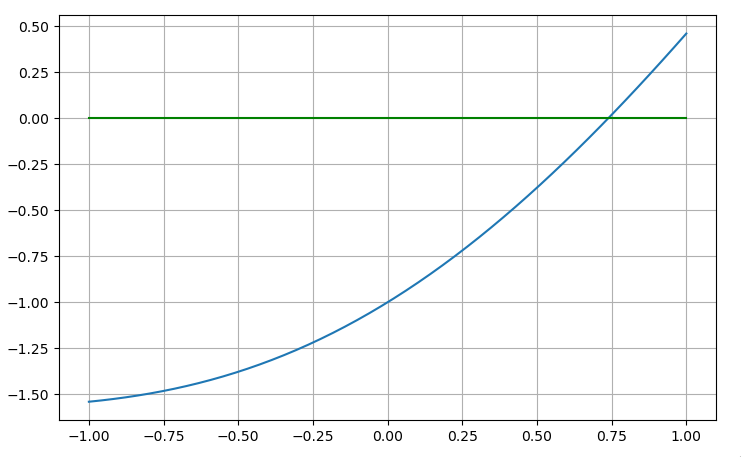
\includegraphics[width=0.5\textwidth]{img/2024-09-23-12-11-58.png}
\end{center}
\subsection{Algoritmo di bisezione}
L'algoritmo di bisezione usa un approccio simile alla ricerca binaria per avvicinarsi sempre di piu' al valore dello zero. Dato in input la funzione continua $ f:\mathbb{R}\to\mathbb{R} $ e un intervallo $ [a,b]. f(a)f(b)<0 $, viene calcolato il valore della funzione nel punto di mezzo $ c $. L'intervallo viene poi ristretto, prendendo $ c $ come uno dei limiti e scegliendo l'altro fra $ a $ e $ b $ in modo che i valori della funzione agli estremi abbiano sempre segno opposto. In pseudocodice:

\begin{algorithm}[H]
\caption{Bisezione semplice}
  \KwIn{$ f: \mathbb{R}\to\mathbb{R} $ continua su $ [a,b] \subset \mathbb{R} $, tale che $ f(a)f(b)<0 $. $ N > 0 $ (numero di iterazioni)}
  \KwOut{Valore approssimato di uno zero di $ f $ su $ [a,b] $}
\SetAlgoLined
\SetNoFillComment
\vspace{3mm}
$c \leftarrow 0$\;
\For{$ N $ times} {
    $ c \gets \frac{a+b}{2} $\;
    \uIf{$ f(a)f(c)<0 $} {
      $ b \gets c $
    }
    \Else {
      $ a \gets c $
    }
}
\Return $ c $
\end{algorithm}

\vspace{3mm}
Se volgiamo assicurarci che il risultato $ r' $ che otteniamo abbia al massimo un errore $ E_{tol} $ rispetto al valore reale $ r $ della radice, basta porre una condizione d'arresto nel ciclo di bisezione. Sapendo che ad ogni ciclo lo zero si trova fra $ a $ e $ b $, scegliendo $ r' $ come punto di mezzo rende l'errore massimo $ E_{max} = \frac{b-a}{2} $, quindi:

\vspace{3mm}
\begin{algorithm}[H]
\caption{Bisezione con errore}
  \KwIn{$ f: \mathbb{R}\to\mathbb{R} $ continua su $ [a,b] \subset \mathbb{R} $, tale che $ f(a)f(b)<0 $. $ E_{tol} $}
  \KwOut{Valore approssimato di uno zero di $ f $ su $ [a,b] $ con errore assoluto al massimo $ E_{tol} $}
\SetAlgoLined
\SetNoFillComment
\vspace{3mm}
$c \leftarrow 0$\;
$ E_{max} = \frac{b-a}{2} $\;
\While{$ E_{max} > E_{tol} $} {
    $ c \gets \frac{a+b}{2} $\;
    \uIf{$ f(a)f(c)<0 $} {
      $ b \gets c $
    }
    \Else {
      $ a \gets c $
    }
    $ E_{max} = \frac{b-a}{2} $
}
\Return $ c $
\end{algorithm}

\section{Iterazione di punto fisso}
Presa la funzione $ f $ di cui vogliamo trovare lo zero, possiamo definire una funzione $ g(x) = x-w(x)f(x) $ dove $ w $ e' una funzione peso \textit{positiva} e \textit{limitata}. Quindi:
\[
  f(x) = 0 \iff g(x) = x
\]

%\begin{figure}[H]
 % \centering
  %\begin{subfigure}[b]{0.45\textwidth}
    no puede soportar este sufrimento
      %%% Creator: Matplotlib, PGF backend
%%
%% To include the figure in your LaTeX document, write
%%   \input{<filename>.pgf}
%%
%% Make sure the required packages are loaded in your preamble
%%   \usepackage{pgf}
%%
%% Also ensure that all the required font packages are loaded; for instance,
%% the lmodern package is sometimes necessary when using math font.
%%   \usepackage{lmodern}
%%
%% Figures using additional raster images can only be included by \input if
%% they are in the same directory as the main LaTeX file. For loading figures
%% from other directories you can use the `import` package
%%   \usepackage{import}
%%
%% and then include the figures with
%%   \import{<path to file>}{<filename>.pgf}
%%
%% Matplotlib used the following preamble
%%   \def\mathdefault#1{#1}
%%   \everymath=\expandafter{\the\everymath\displaystyle}
%%   
%%   \ifdefined\pdftexversion\else  % non-pdftex case.
%%     \usepackage{fontspec}
%%   \fi
%%   \makeatletter\@ifpackageloaded{underscore}{}{\usepackage[strings]{underscore}}\makeatother
%%
\begingroup%
\makeatletter%
\begin{pgfpicture}%
\pgfpathrectangle{\pgfpointorigin}{\pgfqpoint{3.400000in}{1.700000in}}%
\pgfusepath{use as bounding box, clip}%
\begin{pgfscope}%
\pgfsetbuttcap%
\pgfsetmiterjoin%
\definecolor{currentfill}{rgb}{1.000000,1.000000,1.000000}%
\pgfsetfillcolor{currentfill}%
\pgfsetlinewidth{0.000000pt}%
\definecolor{currentstroke}{rgb}{1.000000,1.000000,1.000000}%
\pgfsetstrokecolor{currentstroke}%
\pgfsetdash{}{0pt}%
\pgfpathmoveto{\pgfqpoint{0.000000in}{0.000000in}}%
\pgfpathlineto{\pgfqpoint{3.400000in}{0.000000in}}%
\pgfpathlineto{\pgfqpoint{3.400000in}{1.700000in}}%
\pgfpathlineto{\pgfqpoint{0.000000in}{1.700000in}}%
\pgfpathlineto{\pgfqpoint{0.000000in}{0.000000in}}%
\pgfpathclose%
\pgfusepath{fill}%
\end{pgfscope}%
\begin{pgfscope}%
\pgfsetbuttcap%
\pgfsetmiterjoin%
\definecolor{currentfill}{rgb}{1.000000,1.000000,1.000000}%
\pgfsetfillcolor{currentfill}%
\pgfsetlinewidth{0.000000pt}%
\definecolor{currentstroke}{rgb}{0.000000,0.000000,0.000000}%
\pgfsetstrokecolor{currentstroke}%
\pgfsetstrokeopacity{0.000000}%
\pgfsetdash{}{0pt}%
\pgfpathmoveto{\pgfqpoint{0.425000in}{0.187000in}}%
\pgfpathlineto{\pgfqpoint{3.060000in}{0.187000in}}%
\pgfpathlineto{\pgfqpoint{3.060000in}{1.496000in}}%
\pgfpathlineto{\pgfqpoint{0.425000in}{1.496000in}}%
\pgfpathlineto{\pgfqpoint{0.425000in}{0.187000in}}%
\pgfpathclose%
\pgfusepath{fill}%
\end{pgfscope}%
\begin{pgfscope}%
\pgfpathrectangle{\pgfqpoint{0.425000in}{0.187000in}}{\pgfqpoint{2.635000in}{1.309000in}}%
\pgfusepath{clip}%
\pgfsetrectcap%
\pgfsetroundjoin%
\pgfsetlinewidth{0.803000pt}%
\definecolor{currentstroke}{rgb}{0.690196,0.690196,0.690196}%
\pgfsetstrokecolor{currentstroke}%
\pgfsetdash{}{0pt}%
\pgfpathmoveto{\pgfqpoint{0.544773in}{0.187000in}}%
\pgfpathlineto{\pgfqpoint{0.544773in}{1.496000in}}%
\pgfusepath{stroke}%
\end{pgfscope}%
\begin{pgfscope}%
\pgfsetbuttcap%
\pgfsetroundjoin%
\definecolor{currentfill}{rgb}{0.000000,0.000000,0.000000}%
\pgfsetfillcolor{currentfill}%
\pgfsetlinewidth{0.803000pt}%
\definecolor{currentstroke}{rgb}{0.000000,0.000000,0.000000}%
\pgfsetstrokecolor{currentstroke}%
\pgfsetdash{}{0pt}%
\pgfsys@defobject{currentmarker}{\pgfqpoint{0.000000in}{-0.048611in}}{\pgfqpoint{0.000000in}{0.000000in}}{%
\pgfpathmoveto{\pgfqpoint{0.000000in}{0.000000in}}%
\pgfpathlineto{\pgfqpoint{0.000000in}{-0.048611in}}%
\pgfusepath{stroke,fill}%
}%
\begin{pgfscope}%
\pgfsys@transformshift{0.544773in}{0.187000in}%
\pgfsys@useobject{currentmarker}{}%
\end{pgfscope}%
\end{pgfscope}%
\begin{pgfscope}%
\definecolor{textcolor}{rgb}{0.000000,0.000000,0.000000}%
\pgfsetstrokecolor{textcolor}%
\pgfsetfillcolor{textcolor}%
\pgftext[x=0.544773in,y=0.089778in,,top]{\color{textcolor}{\rmfamily\fontsize{10.000000}{12.000000}\selectfont\catcode`\^=\active\def^{\ifmmode\sp\else\^{}\fi}\catcode`\%=\active\def%{\%}$\mathdefault{\ensuremath{-}1.0}$}}%
\end{pgfscope}%
\begin{pgfscope}%
\pgfpathrectangle{\pgfqpoint{0.425000in}{0.187000in}}{\pgfqpoint{2.635000in}{1.309000in}}%
\pgfusepath{clip}%
\pgfsetrectcap%
\pgfsetroundjoin%
\pgfsetlinewidth{0.803000pt}%
\definecolor{currentstroke}{rgb}{0.690196,0.690196,0.690196}%
\pgfsetstrokecolor{currentstroke}%
\pgfsetdash{}{0pt}%
\pgfpathmoveto{\pgfqpoint{1.143636in}{0.187000in}}%
\pgfpathlineto{\pgfqpoint{1.143636in}{1.496000in}}%
\pgfusepath{stroke}%
\end{pgfscope}%
\begin{pgfscope}%
\pgfsetbuttcap%
\pgfsetroundjoin%
\definecolor{currentfill}{rgb}{0.000000,0.000000,0.000000}%
\pgfsetfillcolor{currentfill}%
\pgfsetlinewidth{0.803000pt}%
\definecolor{currentstroke}{rgb}{0.000000,0.000000,0.000000}%
\pgfsetstrokecolor{currentstroke}%
\pgfsetdash{}{0pt}%
\pgfsys@defobject{currentmarker}{\pgfqpoint{0.000000in}{-0.048611in}}{\pgfqpoint{0.000000in}{0.000000in}}{%
\pgfpathmoveto{\pgfqpoint{0.000000in}{0.000000in}}%
\pgfpathlineto{\pgfqpoint{0.000000in}{-0.048611in}}%
\pgfusepath{stroke,fill}%
}%
\begin{pgfscope}%
\pgfsys@transformshift{1.143636in}{0.187000in}%
\pgfsys@useobject{currentmarker}{}%
\end{pgfscope}%
\end{pgfscope}%
\begin{pgfscope}%
\definecolor{textcolor}{rgb}{0.000000,0.000000,0.000000}%
\pgfsetstrokecolor{textcolor}%
\pgfsetfillcolor{textcolor}%
\pgftext[x=1.143636in,y=0.089778in,,top]{\color{textcolor}{\rmfamily\fontsize{10.000000}{12.000000}\selectfont\catcode`\^=\active\def^{\ifmmode\sp\else\^{}\fi}\catcode`\%=\active\def%{\%}$\mathdefault{\ensuremath{-}0.5}$}}%
\end{pgfscope}%
\begin{pgfscope}%
\pgfpathrectangle{\pgfqpoint{0.425000in}{0.187000in}}{\pgfqpoint{2.635000in}{1.309000in}}%
\pgfusepath{clip}%
\pgfsetrectcap%
\pgfsetroundjoin%
\pgfsetlinewidth{0.803000pt}%
\definecolor{currentstroke}{rgb}{0.690196,0.690196,0.690196}%
\pgfsetstrokecolor{currentstroke}%
\pgfsetdash{}{0pt}%
\pgfpathmoveto{\pgfqpoint{1.742500in}{0.187000in}}%
\pgfpathlineto{\pgfqpoint{1.742500in}{1.496000in}}%
\pgfusepath{stroke}%
\end{pgfscope}%
\begin{pgfscope}%
\pgfsetbuttcap%
\pgfsetroundjoin%
\definecolor{currentfill}{rgb}{0.000000,0.000000,0.000000}%
\pgfsetfillcolor{currentfill}%
\pgfsetlinewidth{0.803000pt}%
\definecolor{currentstroke}{rgb}{0.000000,0.000000,0.000000}%
\pgfsetstrokecolor{currentstroke}%
\pgfsetdash{}{0pt}%
\pgfsys@defobject{currentmarker}{\pgfqpoint{0.000000in}{-0.048611in}}{\pgfqpoint{0.000000in}{0.000000in}}{%
\pgfpathmoveto{\pgfqpoint{0.000000in}{0.000000in}}%
\pgfpathlineto{\pgfqpoint{0.000000in}{-0.048611in}}%
\pgfusepath{stroke,fill}%
}%
\begin{pgfscope}%
\pgfsys@transformshift{1.742500in}{0.187000in}%
\pgfsys@useobject{currentmarker}{}%
\end{pgfscope}%
\end{pgfscope}%
\begin{pgfscope}%
\definecolor{textcolor}{rgb}{0.000000,0.000000,0.000000}%
\pgfsetstrokecolor{textcolor}%
\pgfsetfillcolor{textcolor}%
\pgftext[x=1.742500in,y=0.089778in,,top]{\color{textcolor}{\rmfamily\fontsize{10.000000}{12.000000}\selectfont\catcode`\^=\active\def^{\ifmmode\sp\else\^{}\fi}\catcode`\%=\active\def%{\%}$\mathdefault{0.0}$}}%
\end{pgfscope}%
\begin{pgfscope}%
\pgfpathrectangle{\pgfqpoint{0.425000in}{0.187000in}}{\pgfqpoint{2.635000in}{1.309000in}}%
\pgfusepath{clip}%
\pgfsetrectcap%
\pgfsetroundjoin%
\pgfsetlinewidth{0.803000pt}%
\definecolor{currentstroke}{rgb}{0.690196,0.690196,0.690196}%
\pgfsetstrokecolor{currentstroke}%
\pgfsetdash{}{0pt}%
\pgfpathmoveto{\pgfqpoint{2.341364in}{0.187000in}}%
\pgfpathlineto{\pgfqpoint{2.341364in}{1.496000in}}%
\pgfusepath{stroke}%
\end{pgfscope}%
\begin{pgfscope}%
\pgfsetbuttcap%
\pgfsetroundjoin%
\definecolor{currentfill}{rgb}{0.000000,0.000000,0.000000}%
\pgfsetfillcolor{currentfill}%
\pgfsetlinewidth{0.803000pt}%
\definecolor{currentstroke}{rgb}{0.000000,0.000000,0.000000}%
\pgfsetstrokecolor{currentstroke}%
\pgfsetdash{}{0pt}%
\pgfsys@defobject{currentmarker}{\pgfqpoint{0.000000in}{-0.048611in}}{\pgfqpoint{0.000000in}{0.000000in}}{%
\pgfpathmoveto{\pgfqpoint{0.000000in}{0.000000in}}%
\pgfpathlineto{\pgfqpoint{0.000000in}{-0.048611in}}%
\pgfusepath{stroke,fill}%
}%
\begin{pgfscope}%
\pgfsys@transformshift{2.341364in}{0.187000in}%
\pgfsys@useobject{currentmarker}{}%
\end{pgfscope}%
\end{pgfscope}%
\begin{pgfscope}%
\definecolor{textcolor}{rgb}{0.000000,0.000000,0.000000}%
\pgfsetstrokecolor{textcolor}%
\pgfsetfillcolor{textcolor}%
\pgftext[x=2.341364in,y=0.089778in,,top]{\color{textcolor}{\rmfamily\fontsize{10.000000}{12.000000}\selectfont\catcode`\^=\active\def^{\ifmmode\sp\else\^{}\fi}\catcode`\%=\active\def%{\%}$\mathdefault{0.5}$}}%
\end{pgfscope}%
\begin{pgfscope}%
\pgfpathrectangle{\pgfqpoint{0.425000in}{0.187000in}}{\pgfqpoint{2.635000in}{1.309000in}}%
\pgfusepath{clip}%
\pgfsetrectcap%
\pgfsetroundjoin%
\pgfsetlinewidth{0.803000pt}%
\definecolor{currentstroke}{rgb}{0.690196,0.690196,0.690196}%
\pgfsetstrokecolor{currentstroke}%
\pgfsetdash{}{0pt}%
\pgfpathmoveto{\pgfqpoint{2.940227in}{0.187000in}}%
\pgfpathlineto{\pgfqpoint{2.940227in}{1.496000in}}%
\pgfusepath{stroke}%
\end{pgfscope}%
\begin{pgfscope}%
\pgfsetbuttcap%
\pgfsetroundjoin%
\definecolor{currentfill}{rgb}{0.000000,0.000000,0.000000}%
\pgfsetfillcolor{currentfill}%
\pgfsetlinewidth{0.803000pt}%
\definecolor{currentstroke}{rgb}{0.000000,0.000000,0.000000}%
\pgfsetstrokecolor{currentstroke}%
\pgfsetdash{}{0pt}%
\pgfsys@defobject{currentmarker}{\pgfqpoint{0.000000in}{-0.048611in}}{\pgfqpoint{0.000000in}{0.000000in}}{%
\pgfpathmoveto{\pgfqpoint{0.000000in}{0.000000in}}%
\pgfpathlineto{\pgfqpoint{0.000000in}{-0.048611in}}%
\pgfusepath{stroke,fill}%
}%
\begin{pgfscope}%
\pgfsys@transformshift{2.940227in}{0.187000in}%
\pgfsys@useobject{currentmarker}{}%
\end{pgfscope}%
\end{pgfscope}%
\begin{pgfscope}%
\definecolor{textcolor}{rgb}{0.000000,0.000000,0.000000}%
\pgfsetstrokecolor{textcolor}%
\pgfsetfillcolor{textcolor}%
\pgftext[x=2.940227in,y=0.089778in,,top]{\color{textcolor}{\rmfamily\fontsize{10.000000}{12.000000}\selectfont\catcode`\^=\active\def^{\ifmmode\sp\else\^{}\fi}\catcode`\%=\active\def%{\%}$\mathdefault{1.0}$}}%
\end{pgfscope}%
\begin{pgfscope}%
\pgfpathrectangle{\pgfqpoint{0.425000in}{0.187000in}}{\pgfqpoint{2.635000in}{1.309000in}}%
\pgfusepath{clip}%
\pgfsetrectcap%
\pgfsetroundjoin%
\pgfsetlinewidth{0.803000pt}%
\definecolor{currentstroke}{rgb}{0.690196,0.690196,0.690196}%
\pgfsetstrokecolor{currentstroke}%
\pgfsetdash{}{0pt}%
\pgfpathmoveto{\pgfqpoint{0.425000in}{0.567980in}}%
\pgfpathlineto{\pgfqpoint{3.060000in}{0.567980in}}%
\pgfusepath{stroke}%
\end{pgfscope}%
\begin{pgfscope}%
\pgfsetbuttcap%
\pgfsetroundjoin%
\definecolor{currentfill}{rgb}{0.000000,0.000000,0.000000}%
\pgfsetfillcolor{currentfill}%
\pgfsetlinewidth{0.803000pt}%
\definecolor{currentstroke}{rgb}{0.000000,0.000000,0.000000}%
\pgfsetstrokecolor{currentstroke}%
\pgfsetdash{}{0pt}%
\pgfsys@defobject{currentmarker}{\pgfqpoint{-0.048611in}{0.000000in}}{\pgfqpoint{-0.000000in}{0.000000in}}{%
\pgfpathmoveto{\pgfqpoint{-0.000000in}{0.000000in}}%
\pgfpathlineto{\pgfqpoint{-0.048611in}{0.000000in}}%
\pgfusepath{stroke,fill}%
}%
\begin{pgfscope}%
\pgfsys@transformshift{0.425000in}{0.567980in}%
\pgfsys@useobject{currentmarker}{}%
\end{pgfscope}%
\end{pgfscope}%
\begin{pgfscope}%
\definecolor{textcolor}{rgb}{0.000000,0.000000,0.000000}%
\pgfsetstrokecolor{textcolor}%
\pgfsetfillcolor{textcolor}%
\pgftext[x=0.150308in, y=0.519755in, left, base]{\color{textcolor}{\rmfamily\fontsize{10.000000}{12.000000}\selectfont\catcode`\^=\active\def^{\ifmmode\sp\else\^{}\fi}\catcode`\%=\active\def%{\%}$\mathdefault{\ensuremath{-}1}$}}%
\end{pgfscope}%
\begin{pgfscope}%
\pgfpathrectangle{\pgfqpoint{0.425000in}{0.187000in}}{\pgfqpoint{2.635000in}{1.309000in}}%
\pgfusepath{clip}%
\pgfsetrectcap%
\pgfsetroundjoin%
\pgfsetlinewidth{0.803000pt}%
\definecolor{currentstroke}{rgb}{0.690196,0.690196,0.690196}%
\pgfsetstrokecolor{currentstroke}%
\pgfsetdash{}{0pt}%
\pgfpathmoveto{\pgfqpoint{0.425000in}{1.162980in}}%
\pgfpathlineto{\pgfqpoint{3.060000in}{1.162980in}}%
\pgfusepath{stroke}%
\end{pgfscope}%
\begin{pgfscope}%
\pgfsetbuttcap%
\pgfsetroundjoin%
\definecolor{currentfill}{rgb}{0.000000,0.000000,0.000000}%
\pgfsetfillcolor{currentfill}%
\pgfsetlinewidth{0.803000pt}%
\definecolor{currentstroke}{rgb}{0.000000,0.000000,0.000000}%
\pgfsetstrokecolor{currentstroke}%
\pgfsetdash{}{0pt}%
\pgfsys@defobject{currentmarker}{\pgfqpoint{-0.048611in}{0.000000in}}{\pgfqpoint{-0.000000in}{0.000000in}}{%
\pgfpathmoveto{\pgfqpoint{-0.000000in}{0.000000in}}%
\pgfpathlineto{\pgfqpoint{-0.048611in}{0.000000in}}%
\pgfusepath{stroke,fill}%
}%
\begin{pgfscope}%
\pgfsys@transformshift{0.425000in}{1.162980in}%
\pgfsys@useobject{currentmarker}{}%
\end{pgfscope}%
\end{pgfscope}%
\begin{pgfscope}%
\definecolor{textcolor}{rgb}{0.000000,0.000000,0.000000}%
\pgfsetstrokecolor{textcolor}%
\pgfsetfillcolor{textcolor}%
\pgftext[x=0.258333in, y=1.114755in, left, base]{\color{textcolor}{\rmfamily\fontsize{10.000000}{12.000000}\selectfont\catcode`\^=\active\def^{\ifmmode\sp\else\^{}\fi}\catcode`\%=\active\def%{\%}$\mathdefault{0}$}}%
\end{pgfscope}%
\begin{pgfscope}%
\pgfpathrectangle{\pgfqpoint{0.425000in}{0.187000in}}{\pgfqpoint{2.635000in}{1.309000in}}%
\pgfusepath{clip}%
\pgfsetrectcap%
\pgfsetroundjoin%
\pgfsetlinewidth{1.505625pt}%
\definecolor{currentstroke}{rgb}{0.121569,0.466667,0.705882}%
\pgfsetstrokecolor{currentstroke}%
\pgfsetdash{}{0pt}%
\pgfpathmoveto{\pgfqpoint{0.544773in}{0.246500in}}%
\pgfpathlineto{\pgfqpoint{0.593660in}{0.250623in}}%
\pgfpathlineto{\pgfqpoint{0.642546in}{0.255316in}}%
\pgfpathlineto{\pgfqpoint{0.691433in}{0.260610in}}%
\pgfpathlineto{\pgfqpoint{0.740320in}{0.266538in}}%
\pgfpathlineto{\pgfqpoint{0.789207in}{0.273129in}}%
\pgfpathlineto{\pgfqpoint{0.838094in}{0.280414in}}%
\pgfpathlineto{\pgfqpoint{0.886981in}{0.288421in}}%
\pgfpathlineto{\pgfqpoint{0.935867in}{0.297176in}}%
\pgfpathlineto{\pgfqpoint{0.984754in}{0.306707in}}%
\pgfpathlineto{\pgfqpoint{1.033641in}{0.317036in}}%
\pgfpathlineto{\pgfqpoint{1.082528in}{0.328188in}}%
\pgfpathlineto{\pgfqpoint{1.131415in}{0.340185in}}%
\pgfpathlineto{\pgfqpoint{1.180301in}{0.353046in}}%
\pgfpathlineto{\pgfqpoint{1.229188in}{0.366791in}}%
\pgfpathlineto{\pgfqpoint{1.278075in}{0.381438in}}%
\pgfpathlineto{\pgfqpoint{1.326962in}{0.397003in}}%
\pgfpathlineto{\pgfqpoint{1.375849in}{0.413499in}}%
\pgfpathlineto{\pgfqpoint{1.424736in}{0.430940in}}%
\pgfpathlineto{\pgfqpoint{1.473622in}{0.449338in}}%
\pgfpathlineto{\pgfqpoint{1.522509in}{0.468702in}}%
\pgfpathlineto{\pgfqpoint{1.571396in}{0.489041in}}%
\pgfpathlineto{\pgfqpoint{1.620283in}{0.510361in}}%
\pgfpathlineto{\pgfqpoint{1.669170in}{0.532666in}}%
\pgfpathlineto{\pgfqpoint{1.718057in}{0.555961in}}%
\pgfpathlineto{\pgfqpoint{1.766943in}{0.580247in}}%
\pgfpathlineto{\pgfqpoint{1.815830in}{0.605523in}}%
\pgfpathlineto{\pgfqpoint{1.864717in}{0.631789in}}%
\pgfpathlineto{\pgfqpoint{1.913604in}{0.659041in}}%
\pgfpathlineto{\pgfqpoint{1.962491in}{0.687274in}}%
\pgfpathlineto{\pgfqpoint{2.011378in}{0.716481in}}%
\pgfpathlineto{\pgfqpoint{2.060264in}{0.746655in}}%
\pgfpathlineto{\pgfqpoint{2.109151in}{0.777785in}}%
\pgfpathlineto{\pgfqpoint{2.158038in}{0.809860in}}%
\pgfpathlineto{\pgfqpoint{2.206925in}{0.842867in}}%
\pgfpathlineto{\pgfqpoint{2.255812in}{0.876791in}}%
\pgfpathlineto{\pgfqpoint{2.304699in}{0.911618in}}%
\pgfpathlineto{\pgfqpoint{2.353585in}{0.947328in}}%
\pgfpathlineto{\pgfqpoint{2.402472in}{0.983903in}}%
\pgfpathlineto{\pgfqpoint{2.451359in}{1.021322in}}%
\pgfpathlineto{\pgfqpoint{2.500246in}{1.059564in}}%
\pgfpathlineto{\pgfqpoint{2.549133in}{1.098605in}}%
\pgfpathlineto{\pgfqpoint{2.598019in}{1.138421in}}%
\pgfpathlineto{\pgfqpoint{2.646906in}{1.178986in}}%
\pgfpathlineto{\pgfqpoint{2.695793in}{1.220272in}}%
\pgfpathlineto{\pgfqpoint{2.744680in}{1.262252in}}%
\pgfpathlineto{\pgfqpoint{2.793567in}{1.304896in}}%
\pgfpathlineto{\pgfqpoint{2.842454in}{1.348173in}}%
\pgfpathlineto{\pgfqpoint{2.891340in}{1.392052in}}%
\pgfpathlineto{\pgfqpoint{2.940227in}{1.436500in}}%
\pgfusepath{stroke}%
\end{pgfscope}%
\begin{pgfscope}%
\pgfpathrectangle{\pgfqpoint{0.425000in}{0.187000in}}{\pgfqpoint{2.635000in}{1.309000in}}%
\pgfusepath{clip}%
\pgfsetrectcap%
\pgfsetroundjoin%
\pgfsetlinewidth{1.505625pt}%
\definecolor{currentstroke}{rgb}{1.000000,0.498039,0.054902}%
\pgfsetstrokecolor{currentstroke}%
\pgfsetdash{}{0pt}%
\pgfpathmoveto{\pgfqpoint{0.544773in}{1.162980in}}%
\pgfpathlineto{\pgfqpoint{2.940227in}{1.162980in}}%
\pgfusepath{stroke}%
\end{pgfscope}%
\begin{pgfscope}%
\pgfsetrectcap%
\pgfsetmiterjoin%
\pgfsetlinewidth{0.803000pt}%
\definecolor{currentstroke}{rgb}{0.000000,0.000000,0.000000}%
\pgfsetstrokecolor{currentstroke}%
\pgfsetdash{}{0pt}%
\pgfpathmoveto{\pgfqpoint{0.425000in}{0.187000in}}%
\pgfpathlineto{\pgfqpoint{0.425000in}{1.496000in}}%
\pgfusepath{stroke}%
\end{pgfscope}%
\begin{pgfscope}%
\pgfsetrectcap%
\pgfsetmiterjoin%
\pgfsetlinewidth{0.803000pt}%
\definecolor{currentstroke}{rgb}{0.000000,0.000000,0.000000}%
\pgfsetstrokecolor{currentstroke}%
\pgfsetdash{}{0pt}%
\pgfpathmoveto{\pgfqpoint{3.060000in}{0.187000in}}%
\pgfpathlineto{\pgfqpoint{3.060000in}{1.496000in}}%
\pgfusepath{stroke}%
\end{pgfscope}%
\begin{pgfscope}%
\pgfsetrectcap%
\pgfsetmiterjoin%
\pgfsetlinewidth{0.803000pt}%
\definecolor{currentstroke}{rgb}{0.000000,0.000000,0.000000}%
\pgfsetstrokecolor{currentstroke}%
\pgfsetdash{}{0pt}%
\pgfpathmoveto{\pgfqpoint{0.425000in}{0.187000in}}%
\pgfpathlineto{\pgfqpoint{3.060000in}{0.187000in}}%
\pgfusepath{stroke}%
\end{pgfscope}%
\begin{pgfscope}%
\pgfsetrectcap%
\pgfsetmiterjoin%
\pgfsetlinewidth{0.803000pt}%
\definecolor{currentstroke}{rgb}{0.000000,0.000000,0.000000}%
\pgfsetstrokecolor{currentstroke}%
\pgfsetdash{}{0pt}%
\pgfpathmoveto{\pgfqpoint{0.425000in}{1.496000in}}%
\pgfpathlineto{\pgfqpoint{3.060000in}{1.496000in}}%
\pgfusepath{stroke}%
\end{pgfscope}%
\begin{pgfscope}%
\definecolor{textcolor}{rgb}{0.000000,0.000000,0.000000}%
\pgfsetstrokecolor{textcolor}%
\pgfsetfillcolor{textcolor}%
\pgftext[x=1.742500in,y=1.579333in,,base]{\color{textcolor}{\rmfamily\fontsize{12.000000}{14.400000}\selectfont\catcode`\^=\active\def^{\ifmmode\sp\else\^{}\fi}\catcode`\%=\active\def%{\%}$y = f(x) = x - \cos(x)$ and $y=0$}}%
\end{pgfscope}%
\end{pgfpicture}%
\makeatother%
\endgroup%

  %\end{subfigure}
  %\begin{subfigure}[b]{0.45\textwidth}
   % no puede soportar este sufrimento
      %%% Creator: Matplotlib, PGF backend
%%
%% To include the figure in your LaTeX document, write
%%   \input{<filename>.pgf}
%%
%% Make sure the required packages are loaded in your preamble
%%   \usepackage{pgf}
%%
%% Also ensure that all the required font packages are loaded; for instance,
%% the lmodern package is sometimes necessary when using math font.
%%   \usepackage{lmodern}
%%
%% Figures using additional raster images can only be included by \input if
%% they are in the same directory as the main LaTeX file. For loading figures
%% from other directories you can use the `import` package
%%   \usepackage{import}
%%
%% and then include the figures with
%%   \import{<path to file>}{<filename>.pgf}
%%
%% Matplotlib used the following preamble
%%   \def\mathdefault#1{#1}
%%   \everymath=\expandafter{\the\everymath\displaystyle}
%%   
%%   \ifdefined\pdftexversion\else  % non-pdftex case.
%%     \usepackage{fontspec}
%%   \fi
%%   \makeatletter\@ifpackageloaded{underscore}{}{\usepackage[strings]{underscore}}\makeatother
%%
\begingroup%
\makeatletter%
\begin{pgfpicture}%
\pgfpathrectangle{\pgfpointorigin}{\pgfqpoint{5.000000in}{2.500000in}}%
\pgfusepath{use as bounding box, clip}%
\begin{pgfscope}%
\pgfsetbuttcap%
\pgfsetmiterjoin%
\definecolor{currentfill}{rgb}{1.000000,1.000000,1.000000}%
\pgfsetfillcolor{currentfill}%
\pgfsetlinewidth{0.000000pt}%
\definecolor{currentstroke}{rgb}{1.000000,1.000000,1.000000}%
\pgfsetstrokecolor{currentstroke}%
\pgfsetdash{}{0pt}%
\pgfpathmoveto{\pgfqpoint{0.000000in}{0.000000in}}%
\pgfpathlineto{\pgfqpoint{5.000000in}{0.000000in}}%
\pgfpathlineto{\pgfqpoint{5.000000in}{2.500000in}}%
\pgfpathlineto{\pgfqpoint{0.000000in}{2.500000in}}%
\pgfpathlineto{\pgfqpoint{0.000000in}{0.000000in}}%
\pgfpathclose%
\pgfusepath{fill}%
\end{pgfscope}%
\begin{pgfscope}%
\pgfsetbuttcap%
\pgfsetmiterjoin%
\definecolor{currentfill}{rgb}{1.000000,1.000000,1.000000}%
\pgfsetfillcolor{currentfill}%
\pgfsetlinewidth{0.000000pt}%
\definecolor{currentstroke}{rgb}{0.000000,0.000000,0.000000}%
\pgfsetstrokecolor{currentstroke}%
\pgfsetstrokeopacity{0.000000}%
\pgfsetdash{}{0pt}%
\pgfpathmoveto{\pgfqpoint{0.625000in}{0.275000in}}%
\pgfpathlineto{\pgfqpoint{4.500000in}{0.275000in}}%
\pgfpathlineto{\pgfqpoint{4.500000in}{2.200000in}}%
\pgfpathlineto{\pgfqpoint{0.625000in}{2.200000in}}%
\pgfpathlineto{\pgfqpoint{0.625000in}{0.275000in}}%
\pgfpathclose%
\pgfusepath{fill}%
\end{pgfscope}%
\begin{pgfscope}%
\pgfpathrectangle{\pgfqpoint{0.625000in}{0.275000in}}{\pgfqpoint{3.875000in}{1.925000in}}%
\pgfusepath{clip}%
\pgfsetrectcap%
\pgfsetroundjoin%
\pgfsetlinewidth{0.803000pt}%
\definecolor{currentstroke}{rgb}{0.690196,0.690196,0.690196}%
\pgfsetstrokecolor{currentstroke}%
\pgfsetdash{}{0pt}%
\pgfpathmoveto{\pgfqpoint{0.801136in}{0.275000in}}%
\pgfpathlineto{\pgfqpoint{0.801136in}{2.200000in}}%
\pgfusepath{stroke}%
\end{pgfscope}%
\begin{pgfscope}%
\pgfsetbuttcap%
\pgfsetroundjoin%
\definecolor{currentfill}{rgb}{0.000000,0.000000,0.000000}%
\pgfsetfillcolor{currentfill}%
\pgfsetlinewidth{0.803000pt}%
\definecolor{currentstroke}{rgb}{0.000000,0.000000,0.000000}%
\pgfsetstrokecolor{currentstroke}%
\pgfsetdash{}{0pt}%
\pgfsys@defobject{currentmarker}{\pgfqpoint{0.000000in}{-0.048611in}}{\pgfqpoint{0.000000in}{0.000000in}}{%
\pgfpathmoveto{\pgfqpoint{0.000000in}{0.000000in}}%
\pgfpathlineto{\pgfqpoint{0.000000in}{-0.048611in}}%
\pgfusepath{stroke,fill}%
}%
\begin{pgfscope}%
\pgfsys@transformshift{0.801136in}{0.275000in}%
\pgfsys@useobject{currentmarker}{}%
\end{pgfscope}%
\end{pgfscope}%
\begin{pgfscope}%
\definecolor{textcolor}{rgb}{0.000000,0.000000,0.000000}%
\pgfsetstrokecolor{textcolor}%
\pgfsetfillcolor{textcolor}%
\pgftext[x=0.801136in,y=0.177778in,,top]{\color{textcolor}{\rmfamily\fontsize{10.000000}{12.000000}\selectfont\catcode`\^=\active\def^{\ifmmode\sp\else\^{}\fi}\catcode`\%=\active\def%{\%}$\mathdefault{\ensuremath{-}1.00}$}}%
\end{pgfscope}%
\begin{pgfscope}%
\pgfpathrectangle{\pgfqpoint{0.625000in}{0.275000in}}{\pgfqpoint{3.875000in}{1.925000in}}%
\pgfusepath{clip}%
\pgfsetrectcap%
\pgfsetroundjoin%
\pgfsetlinewidth{0.803000pt}%
\definecolor{currentstroke}{rgb}{0.690196,0.690196,0.690196}%
\pgfsetstrokecolor{currentstroke}%
\pgfsetdash{}{0pt}%
\pgfpathmoveto{\pgfqpoint{1.241477in}{0.275000in}}%
\pgfpathlineto{\pgfqpoint{1.241477in}{2.200000in}}%
\pgfusepath{stroke}%
\end{pgfscope}%
\begin{pgfscope}%
\pgfsetbuttcap%
\pgfsetroundjoin%
\definecolor{currentfill}{rgb}{0.000000,0.000000,0.000000}%
\pgfsetfillcolor{currentfill}%
\pgfsetlinewidth{0.803000pt}%
\definecolor{currentstroke}{rgb}{0.000000,0.000000,0.000000}%
\pgfsetstrokecolor{currentstroke}%
\pgfsetdash{}{0pt}%
\pgfsys@defobject{currentmarker}{\pgfqpoint{0.000000in}{-0.048611in}}{\pgfqpoint{0.000000in}{0.000000in}}{%
\pgfpathmoveto{\pgfqpoint{0.000000in}{0.000000in}}%
\pgfpathlineto{\pgfqpoint{0.000000in}{-0.048611in}}%
\pgfusepath{stroke,fill}%
}%
\begin{pgfscope}%
\pgfsys@transformshift{1.241477in}{0.275000in}%
\pgfsys@useobject{currentmarker}{}%
\end{pgfscope}%
\end{pgfscope}%
\begin{pgfscope}%
\definecolor{textcolor}{rgb}{0.000000,0.000000,0.000000}%
\pgfsetstrokecolor{textcolor}%
\pgfsetfillcolor{textcolor}%
\pgftext[x=1.241477in,y=0.177778in,,top]{\color{textcolor}{\rmfamily\fontsize{10.000000}{12.000000}\selectfont\catcode`\^=\active\def^{\ifmmode\sp\else\^{}\fi}\catcode`\%=\active\def%{\%}$\mathdefault{\ensuremath{-}0.75}$}}%
\end{pgfscope}%
\begin{pgfscope}%
\pgfpathrectangle{\pgfqpoint{0.625000in}{0.275000in}}{\pgfqpoint{3.875000in}{1.925000in}}%
\pgfusepath{clip}%
\pgfsetrectcap%
\pgfsetroundjoin%
\pgfsetlinewidth{0.803000pt}%
\definecolor{currentstroke}{rgb}{0.690196,0.690196,0.690196}%
\pgfsetstrokecolor{currentstroke}%
\pgfsetdash{}{0pt}%
\pgfpathmoveto{\pgfqpoint{1.681818in}{0.275000in}}%
\pgfpathlineto{\pgfqpoint{1.681818in}{2.200000in}}%
\pgfusepath{stroke}%
\end{pgfscope}%
\begin{pgfscope}%
\pgfsetbuttcap%
\pgfsetroundjoin%
\definecolor{currentfill}{rgb}{0.000000,0.000000,0.000000}%
\pgfsetfillcolor{currentfill}%
\pgfsetlinewidth{0.803000pt}%
\definecolor{currentstroke}{rgb}{0.000000,0.000000,0.000000}%
\pgfsetstrokecolor{currentstroke}%
\pgfsetdash{}{0pt}%
\pgfsys@defobject{currentmarker}{\pgfqpoint{0.000000in}{-0.048611in}}{\pgfqpoint{0.000000in}{0.000000in}}{%
\pgfpathmoveto{\pgfqpoint{0.000000in}{0.000000in}}%
\pgfpathlineto{\pgfqpoint{0.000000in}{-0.048611in}}%
\pgfusepath{stroke,fill}%
}%
\begin{pgfscope}%
\pgfsys@transformshift{1.681818in}{0.275000in}%
\pgfsys@useobject{currentmarker}{}%
\end{pgfscope}%
\end{pgfscope}%
\begin{pgfscope}%
\definecolor{textcolor}{rgb}{0.000000,0.000000,0.000000}%
\pgfsetstrokecolor{textcolor}%
\pgfsetfillcolor{textcolor}%
\pgftext[x=1.681818in,y=0.177778in,,top]{\color{textcolor}{\rmfamily\fontsize{10.000000}{12.000000}\selectfont\catcode`\^=\active\def^{\ifmmode\sp\else\^{}\fi}\catcode`\%=\active\def%{\%}$\mathdefault{\ensuremath{-}0.50}$}}%
\end{pgfscope}%
\begin{pgfscope}%
\pgfpathrectangle{\pgfqpoint{0.625000in}{0.275000in}}{\pgfqpoint{3.875000in}{1.925000in}}%
\pgfusepath{clip}%
\pgfsetrectcap%
\pgfsetroundjoin%
\pgfsetlinewidth{0.803000pt}%
\definecolor{currentstroke}{rgb}{0.690196,0.690196,0.690196}%
\pgfsetstrokecolor{currentstroke}%
\pgfsetdash{}{0pt}%
\pgfpathmoveto{\pgfqpoint{2.122159in}{0.275000in}}%
\pgfpathlineto{\pgfqpoint{2.122159in}{2.200000in}}%
\pgfusepath{stroke}%
\end{pgfscope}%
\begin{pgfscope}%
\pgfsetbuttcap%
\pgfsetroundjoin%
\definecolor{currentfill}{rgb}{0.000000,0.000000,0.000000}%
\pgfsetfillcolor{currentfill}%
\pgfsetlinewidth{0.803000pt}%
\definecolor{currentstroke}{rgb}{0.000000,0.000000,0.000000}%
\pgfsetstrokecolor{currentstroke}%
\pgfsetdash{}{0pt}%
\pgfsys@defobject{currentmarker}{\pgfqpoint{0.000000in}{-0.048611in}}{\pgfqpoint{0.000000in}{0.000000in}}{%
\pgfpathmoveto{\pgfqpoint{0.000000in}{0.000000in}}%
\pgfpathlineto{\pgfqpoint{0.000000in}{-0.048611in}}%
\pgfusepath{stroke,fill}%
}%
\begin{pgfscope}%
\pgfsys@transformshift{2.122159in}{0.275000in}%
\pgfsys@useobject{currentmarker}{}%
\end{pgfscope}%
\end{pgfscope}%
\begin{pgfscope}%
\definecolor{textcolor}{rgb}{0.000000,0.000000,0.000000}%
\pgfsetstrokecolor{textcolor}%
\pgfsetfillcolor{textcolor}%
\pgftext[x=2.122159in,y=0.177778in,,top]{\color{textcolor}{\rmfamily\fontsize{10.000000}{12.000000}\selectfont\catcode`\^=\active\def^{\ifmmode\sp\else\^{}\fi}\catcode`\%=\active\def%{\%}$\mathdefault{\ensuremath{-}0.25}$}}%
\end{pgfscope}%
\begin{pgfscope}%
\pgfpathrectangle{\pgfqpoint{0.625000in}{0.275000in}}{\pgfqpoint{3.875000in}{1.925000in}}%
\pgfusepath{clip}%
\pgfsetrectcap%
\pgfsetroundjoin%
\pgfsetlinewidth{0.803000pt}%
\definecolor{currentstroke}{rgb}{0.690196,0.690196,0.690196}%
\pgfsetstrokecolor{currentstroke}%
\pgfsetdash{}{0pt}%
\pgfpathmoveto{\pgfqpoint{2.562500in}{0.275000in}}%
\pgfpathlineto{\pgfqpoint{2.562500in}{2.200000in}}%
\pgfusepath{stroke}%
\end{pgfscope}%
\begin{pgfscope}%
\pgfsetbuttcap%
\pgfsetroundjoin%
\definecolor{currentfill}{rgb}{0.000000,0.000000,0.000000}%
\pgfsetfillcolor{currentfill}%
\pgfsetlinewidth{0.803000pt}%
\definecolor{currentstroke}{rgb}{0.000000,0.000000,0.000000}%
\pgfsetstrokecolor{currentstroke}%
\pgfsetdash{}{0pt}%
\pgfsys@defobject{currentmarker}{\pgfqpoint{0.000000in}{-0.048611in}}{\pgfqpoint{0.000000in}{0.000000in}}{%
\pgfpathmoveto{\pgfqpoint{0.000000in}{0.000000in}}%
\pgfpathlineto{\pgfqpoint{0.000000in}{-0.048611in}}%
\pgfusepath{stroke,fill}%
}%
\begin{pgfscope}%
\pgfsys@transformshift{2.562500in}{0.275000in}%
\pgfsys@useobject{currentmarker}{}%
\end{pgfscope}%
\end{pgfscope}%
\begin{pgfscope}%
\definecolor{textcolor}{rgb}{0.000000,0.000000,0.000000}%
\pgfsetstrokecolor{textcolor}%
\pgfsetfillcolor{textcolor}%
\pgftext[x=2.562500in,y=0.177778in,,top]{\color{textcolor}{\rmfamily\fontsize{10.000000}{12.000000}\selectfont\catcode`\^=\active\def^{\ifmmode\sp\else\^{}\fi}\catcode`\%=\active\def%{\%}$\mathdefault{0.00}$}}%
\end{pgfscope}%
\begin{pgfscope}%
\pgfpathrectangle{\pgfqpoint{0.625000in}{0.275000in}}{\pgfqpoint{3.875000in}{1.925000in}}%
\pgfusepath{clip}%
\pgfsetrectcap%
\pgfsetroundjoin%
\pgfsetlinewidth{0.803000pt}%
\definecolor{currentstroke}{rgb}{0.690196,0.690196,0.690196}%
\pgfsetstrokecolor{currentstroke}%
\pgfsetdash{}{0pt}%
\pgfpathmoveto{\pgfqpoint{3.002841in}{0.275000in}}%
\pgfpathlineto{\pgfqpoint{3.002841in}{2.200000in}}%
\pgfusepath{stroke}%
\end{pgfscope}%
\begin{pgfscope}%
\pgfsetbuttcap%
\pgfsetroundjoin%
\definecolor{currentfill}{rgb}{0.000000,0.000000,0.000000}%
\pgfsetfillcolor{currentfill}%
\pgfsetlinewidth{0.803000pt}%
\definecolor{currentstroke}{rgb}{0.000000,0.000000,0.000000}%
\pgfsetstrokecolor{currentstroke}%
\pgfsetdash{}{0pt}%
\pgfsys@defobject{currentmarker}{\pgfqpoint{0.000000in}{-0.048611in}}{\pgfqpoint{0.000000in}{0.000000in}}{%
\pgfpathmoveto{\pgfqpoint{0.000000in}{0.000000in}}%
\pgfpathlineto{\pgfqpoint{0.000000in}{-0.048611in}}%
\pgfusepath{stroke,fill}%
}%
\begin{pgfscope}%
\pgfsys@transformshift{3.002841in}{0.275000in}%
\pgfsys@useobject{currentmarker}{}%
\end{pgfscope}%
\end{pgfscope}%
\begin{pgfscope}%
\definecolor{textcolor}{rgb}{0.000000,0.000000,0.000000}%
\pgfsetstrokecolor{textcolor}%
\pgfsetfillcolor{textcolor}%
\pgftext[x=3.002841in,y=0.177778in,,top]{\color{textcolor}{\rmfamily\fontsize{10.000000}{12.000000}\selectfont\catcode`\^=\active\def^{\ifmmode\sp\else\^{}\fi}\catcode`\%=\active\def%{\%}$\mathdefault{0.25}$}}%
\end{pgfscope}%
\begin{pgfscope}%
\pgfpathrectangle{\pgfqpoint{0.625000in}{0.275000in}}{\pgfqpoint{3.875000in}{1.925000in}}%
\pgfusepath{clip}%
\pgfsetrectcap%
\pgfsetroundjoin%
\pgfsetlinewidth{0.803000pt}%
\definecolor{currentstroke}{rgb}{0.690196,0.690196,0.690196}%
\pgfsetstrokecolor{currentstroke}%
\pgfsetdash{}{0pt}%
\pgfpathmoveto{\pgfqpoint{3.443182in}{0.275000in}}%
\pgfpathlineto{\pgfqpoint{3.443182in}{2.200000in}}%
\pgfusepath{stroke}%
\end{pgfscope}%
\begin{pgfscope}%
\pgfsetbuttcap%
\pgfsetroundjoin%
\definecolor{currentfill}{rgb}{0.000000,0.000000,0.000000}%
\pgfsetfillcolor{currentfill}%
\pgfsetlinewidth{0.803000pt}%
\definecolor{currentstroke}{rgb}{0.000000,0.000000,0.000000}%
\pgfsetstrokecolor{currentstroke}%
\pgfsetdash{}{0pt}%
\pgfsys@defobject{currentmarker}{\pgfqpoint{0.000000in}{-0.048611in}}{\pgfqpoint{0.000000in}{0.000000in}}{%
\pgfpathmoveto{\pgfqpoint{0.000000in}{0.000000in}}%
\pgfpathlineto{\pgfqpoint{0.000000in}{-0.048611in}}%
\pgfusepath{stroke,fill}%
}%
\begin{pgfscope}%
\pgfsys@transformshift{3.443182in}{0.275000in}%
\pgfsys@useobject{currentmarker}{}%
\end{pgfscope}%
\end{pgfscope}%
\begin{pgfscope}%
\definecolor{textcolor}{rgb}{0.000000,0.000000,0.000000}%
\pgfsetstrokecolor{textcolor}%
\pgfsetfillcolor{textcolor}%
\pgftext[x=3.443182in,y=0.177778in,,top]{\color{textcolor}{\rmfamily\fontsize{10.000000}{12.000000}\selectfont\catcode`\^=\active\def^{\ifmmode\sp\else\^{}\fi}\catcode`\%=\active\def%{\%}$\mathdefault{0.50}$}}%
\end{pgfscope}%
\begin{pgfscope}%
\pgfpathrectangle{\pgfqpoint{0.625000in}{0.275000in}}{\pgfqpoint{3.875000in}{1.925000in}}%
\pgfusepath{clip}%
\pgfsetrectcap%
\pgfsetroundjoin%
\pgfsetlinewidth{0.803000pt}%
\definecolor{currentstroke}{rgb}{0.690196,0.690196,0.690196}%
\pgfsetstrokecolor{currentstroke}%
\pgfsetdash{}{0pt}%
\pgfpathmoveto{\pgfqpoint{3.883523in}{0.275000in}}%
\pgfpathlineto{\pgfqpoint{3.883523in}{2.200000in}}%
\pgfusepath{stroke}%
\end{pgfscope}%
\begin{pgfscope}%
\pgfsetbuttcap%
\pgfsetroundjoin%
\definecolor{currentfill}{rgb}{0.000000,0.000000,0.000000}%
\pgfsetfillcolor{currentfill}%
\pgfsetlinewidth{0.803000pt}%
\definecolor{currentstroke}{rgb}{0.000000,0.000000,0.000000}%
\pgfsetstrokecolor{currentstroke}%
\pgfsetdash{}{0pt}%
\pgfsys@defobject{currentmarker}{\pgfqpoint{0.000000in}{-0.048611in}}{\pgfqpoint{0.000000in}{0.000000in}}{%
\pgfpathmoveto{\pgfqpoint{0.000000in}{0.000000in}}%
\pgfpathlineto{\pgfqpoint{0.000000in}{-0.048611in}}%
\pgfusepath{stroke,fill}%
}%
\begin{pgfscope}%
\pgfsys@transformshift{3.883523in}{0.275000in}%
\pgfsys@useobject{currentmarker}{}%
\end{pgfscope}%
\end{pgfscope}%
\begin{pgfscope}%
\definecolor{textcolor}{rgb}{0.000000,0.000000,0.000000}%
\pgfsetstrokecolor{textcolor}%
\pgfsetfillcolor{textcolor}%
\pgftext[x=3.883523in,y=0.177778in,,top]{\color{textcolor}{\rmfamily\fontsize{10.000000}{12.000000}\selectfont\catcode`\^=\active\def^{\ifmmode\sp\else\^{}\fi}\catcode`\%=\active\def%{\%}$\mathdefault{0.75}$}}%
\end{pgfscope}%
\begin{pgfscope}%
\pgfpathrectangle{\pgfqpoint{0.625000in}{0.275000in}}{\pgfqpoint{3.875000in}{1.925000in}}%
\pgfusepath{clip}%
\pgfsetrectcap%
\pgfsetroundjoin%
\pgfsetlinewidth{0.803000pt}%
\definecolor{currentstroke}{rgb}{0.690196,0.690196,0.690196}%
\pgfsetstrokecolor{currentstroke}%
\pgfsetdash{}{0pt}%
\pgfpathmoveto{\pgfqpoint{4.323864in}{0.275000in}}%
\pgfpathlineto{\pgfqpoint{4.323864in}{2.200000in}}%
\pgfusepath{stroke}%
\end{pgfscope}%
\begin{pgfscope}%
\pgfsetbuttcap%
\pgfsetroundjoin%
\definecolor{currentfill}{rgb}{0.000000,0.000000,0.000000}%
\pgfsetfillcolor{currentfill}%
\pgfsetlinewidth{0.803000pt}%
\definecolor{currentstroke}{rgb}{0.000000,0.000000,0.000000}%
\pgfsetstrokecolor{currentstroke}%
\pgfsetdash{}{0pt}%
\pgfsys@defobject{currentmarker}{\pgfqpoint{0.000000in}{-0.048611in}}{\pgfqpoint{0.000000in}{0.000000in}}{%
\pgfpathmoveto{\pgfqpoint{0.000000in}{0.000000in}}%
\pgfpathlineto{\pgfqpoint{0.000000in}{-0.048611in}}%
\pgfusepath{stroke,fill}%
}%
\begin{pgfscope}%
\pgfsys@transformshift{4.323864in}{0.275000in}%
\pgfsys@useobject{currentmarker}{}%
\end{pgfscope}%
\end{pgfscope}%
\begin{pgfscope}%
\definecolor{textcolor}{rgb}{0.000000,0.000000,0.000000}%
\pgfsetstrokecolor{textcolor}%
\pgfsetfillcolor{textcolor}%
\pgftext[x=4.323864in,y=0.177778in,,top]{\color{textcolor}{\rmfamily\fontsize{10.000000}{12.000000}\selectfont\catcode`\^=\active\def^{\ifmmode\sp\else\^{}\fi}\catcode`\%=\active\def%{\%}$\mathdefault{1.00}$}}%
\end{pgfscope}%
\begin{pgfscope}%
\pgfpathrectangle{\pgfqpoint{0.625000in}{0.275000in}}{\pgfqpoint{3.875000in}{1.925000in}}%
\pgfusepath{clip}%
\pgfsetrectcap%
\pgfsetroundjoin%
\pgfsetlinewidth{0.803000pt}%
\definecolor{currentstroke}{rgb}{0.690196,0.690196,0.690196}%
\pgfsetstrokecolor{currentstroke}%
\pgfsetdash{}{0pt}%
\pgfpathmoveto{\pgfqpoint{0.625000in}{0.362500in}}%
\pgfpathlineto{\pgfqpoint{4.500000in}{0.362500in}}%
\pgfusepath{stroke}%
\end{pgfscope}%
\begin{pgfscope}%
\pgfsetbuttcap%
\pgfsetroundjoin%
\definecolor{currentfill}{rgb}{0.000000,0.000000,0.000000}%
\pgfsetfillcolor{currentfill}%
\pgfsetlinewidth{0.803000pt}%
\definecolor{currentstroke}{rgb}{0.000000,0.000000,0.000000}%
\pgfsetstrokecolor{currentstroke}%
\pgfsetdash{}{0pt}%
\pgfsys@defobject{currentmarker}{\pgfqpoint{-0.048611in}{0.000000in}}{\pgfqpoint{-0.000000in}{0.000000in}}{%
\pgfpathmoveto{\pgfqpoint{-0.000000in}{0.000000in}}%
\pgfpathlineto{\pgfqpoint{-0.048611in}{0.000000in}}%
\pgfusepath{stroke,fill}%
}%
\begin{pgfscope}%
\pgfsys@transformshift{0.625000in}{0.362500in}%
\pgfsys@useobject{currentmarker}{}%
\end{pgfscope}%
\end{pgfscope}%
\begin{pgfscope}%
\definecolor{textcolor}{rgb}{0.000000,0.000000,0.000000}%
\pgfsetstrokecolor{textcolor}%
\pgfsetfillcolor{textcolor}%
\pgftext[x=0.242283in, y=0.314275in, left, base]{\color{textcolor}{\rmfamily\fontsize{10.000000}{12.000000}\selectfont\catcode`\^=\active\def^{\ifmmode\sp\else\^{}\fi}\catcode`\%=\active\def%{\%}$\mathdefault{\ensuremath{-}1.0}$}}%
\end{pgfscope}%
\begin{pgfscope}%
\pgfpathrectangle{\pgfqpoint{0.625000in}{0.275000in}}{\pgfqpoint{3.875000in}{1.925000in}}%
\pgfusepath{clip}%
\pgfsetrectcap%
\pgfsetroundjoin%
\pgfsetlinewidth{0.803000pt}%
\definecolor{currentstroke}{rgb}{0.690196,0.690196,0.690196}%
\pgfsetstrokecolor{currentstroke}%
\pgfsetdash{}{0pt}%
\pgfpathmoveto{\pgfqpoint{0.625000in}{0.800000in}}%
\pgfpathlineto{\pgfqpoint{4.500000in}{0.800000in}}%
\pgfusepath{stroke}%
\end{pgfscope}%
\begin{pgfscope}%
\pgfsetbuttcap%
\pgfsetroundjoin%
\definecolor{currentfill}{rgb}{0.000000,0.000000,0.000000}%
\pgfsetfillcolor{currentfill}%
\pgfsetlinewidth{0.803000pt}%
\definecolor{currentstroke}{rgb}{0.000000,0.000000,0.000000}%
\pgfsetstrokecolor{currentstroke}%
\pgfsetdash{}{0pt}%
\pgfsys@defobject{currentmarker}{\pgfqpoint{-0.048611in}{0.000000in}}{\pgfqpoint{-0.000000in}{0.000000in}}{%
\pgfpathmoveto{\pgfqpoint{-0.000000in}{0.000000in}}%
\pgfpathlineto{\pgfqpoint{-0.048611in}{0.000000in}}%
\pgfusepath{stroke,fill}%
}%
\begin{pgfscope}%
\pgfsys@transformshift{0.625000in}{0.800000in}%
\pgfsys@useobject{currentmarker}{}%
\end{pgfscope}%
\end{pgfscope}%
\begin{pgfscope}%
\definecolor{textcolor}{rgb}{0.000000,0.000000,0.000000}%
\pgfsetstrokecolor{textcolor}%
\pgfsetfillcolor{textcolor}%
\pgftext[x=0.242283in, y=0.751775in, left, base]{\color{textcolor}{\rmfamily\fontsize{10.000000}{12.000000}\selectfont\catcode`\^=\active\def^{\ifmmode\sp\else\^{}\fi}\catcode`\%=\active\def%{\%}$\mathdefault{\ensuremath{-}0.5}$}}%
\end{pgfscope}%
\begin{pgfscope}%
\pgfpathrectangle{\pgfqpoint{0.625000in}{0.275000in}}{\pgfqpoint{3.875000in}{1.925000in}}%
\pgfusepath{clip}%
\pgfsetrectcap%
\pgfsetroundjoin%
\pgfsetlinewidth{0.803000pt}%
\definecolor{currentstroke}{rgb}{0.690196,0.690196,0.690196}%
\pgfsetstrokecolor{currentstroke}%
\pgfsetdash{}{0pt}%
\pgfpathmoveto{\pgfqpoint{0.625000in}{1.237500in}}%
\pgfpathlineto{\pgfqpoint{4.500000in}{1.237500in}}%
\pgfusepath{stroke}%
\end{pgfscope}%
\begin{pgfscope}%
\pgfsetbuttcap%
\pgfsetroundjoin%
\definecolor{currentfill}{rgb}{0.000000,0.000000,0.000000}%
\pgfsetfillcolor{currentfill}%
\pgfsetlinewidth{0.803000pt}%
\definecolor{currentstroke}{rgb}{0.000000,0.000000,0.000000}%
\pgfsetstrokecolor{currentstroke}%
\pgfsetdash{}{0pt}%
\pgfsys@defobject{currentmarker}{\pgfqpoint{-0.048611in}{0.000000in}}{\pgfqpoint{-0.000000in}{0.000000in}}{%
\pgfpathmoveto{\pgfqpoint{-0.000000in}{0.000000in}}%
\pgfpathlineto{\pgfqpoint{-0.048611in}{0.000000in}}%
\pgfusepath{stroke,fill}%
}%
\begin{pgfscope}%
\pgfsys@transformshift{0.625000in}{1.237500in}%
\pgfsys@useobject{currentmarker}{}%
\end{pgfscope}%
\end{pgfscope}%
\begin{pgfscope}%
\definecolor{textcolor}{rgb}{0.000000,0.000000,0.000000}%
\pgfsetstrokecolor{textcolor}%
\pgfsetfillcolor{textcolor}%
\pgftext[x=0.350308in, y=1.189275in, left, base]{\color{textcolor}{\rmfamily\fontsize{10.000000}{12.000000}\selectfont\catcode`\^=\active\def^{\ifmmode\sp\else\^{}\fi}\catcode`\%=\active\def%{\%}$\mathdefault{0.0}$}}%
\end{pgfscope}%
\begin{pgfscope}%
\pgfpathrectangle{\pgfqpoint{0.625000in}{0.275000in}}{\pgfqpoint{3.875000in}{1.925000in}}%
\pgfusepath{clip}%
\pgfsetrectcap%
\pgfsetroundjoin%
\pgfsetlinewidth{0.803000pt}%
\definecolor{currentstroke}{rgb}{0.690196,0.690196,0.690196}%
\pgfsetstrokecolor{currentstroke}%
\pgfsetdash{}{0pt}%
\pgfpathmoveto{\pgfqpoint{0.625000in}{1.675000in}}%
\pgfpathlineto{\pgfqpoint{4.500000in}{1.675000in}}%
\pgfusepath{stroke}%
\end{pgfscope}%
\begin{pgfscope}%
\pgfsetbuttcap%
\pgfsetroundjoin%
\definecolor{currentfill}{rgb}{0.000000,0.000000,0.000000}%
\pgfsetfillcolor{currentfill}%
\pgfsetlinewidth{0.803000pt}%
\definecolor{currentstroke}{rgb}{0.000000,0.000000,0.000000}%
\pgfsetstrokecolor{currentstroke}%
\pgfsetdash{}{0pt}%
\pgfsys@defobject{currentmarker}{\pgfqpoint{-0.048611in}{0.000000in}}{\pgfqpoint{-0.000000in}{0.000000in}}{%
\pgfpathmoveto{\pgfqpoint{-0.000000in}{0.000000in}}%
\pgfpathlineto{\pgfqpoint{-0.048611in}{0.000000in}}%
\pgfusepath{stroke,fill}%
}%
\begin{pgfscope}%
\pgfsys@transformshift{0.625000in}{1.675000in}%
\pgfsys@useobject{currentmarker}{}%
\end{pgfscope}%
\end{pgfscope}%
\begin{pgfscope}%
\definecolor{textcolor}{rgb}{0.000000,0.000000,0.000000}%
\pgfsetstrokecolor{textcolor}%
\pgfsetfillcolor{textcolor}%
\pgftext[x=0.350308in, y=1.626775in, left, base]{\color{textcolor}{\rmfamily\fontsize{10.000000}{12.000000}\selectfont\catcode`\^=\active\def^{\ifmmode\sp\else\^{}\fi}\catcode`\%=\active\def%{\%}$\mathdefault{0.5}$}}%
\end{pgfscope}%
\begin{pgfscope}%
\pgfpathrectangle{\pgfqpoint{0.625000in}{0.275000in}}{\pgfqpoint{3.875000in}{1.925000in}}%
\pgfusepath{clip}%
\pgfsetrectcap%
\pgfsetroundjoin%
\pgfsetlinewidth{0.803000pt}%
\definecolor{currentstroke}{rgb}{0.690196,0.690196,0.690196}%
\pgfsetstrokecolor{currentstroke}%
\pgfsetdash{}{0pt}%
\pgfpathmoveto{\pgfqpoint{0.625000in}{2.112500in}}%
\pgfpathlineto{\pgfqpoint{4.500000in}{2.112500in}}%
\pgfusepath{stroke}%
\end{pgfscope}%
\begin{pgfscope}%
\pgfsetbuttcap%
\pgfsetroundjoin%
\definecolor{currentfill}{rgb}{0.000000,0.000000,0.000000}%
\pgfsetfillcolor{currentfill}%
\pgfsetlinewidth{0.803000pt}%
\definecolor{currentstroke}{rgb}{0.000000,0.000000,0.000000}%
\pgfsetstrokecolor{currentstroke}%
\pgfsetdash{}{0pt}%
\pgfsys@defobject{currentmarker}{\pgfqpoint{-0.048611in}{0.000000in}}{\pgfqpoint{-0.000000in}{0.000000in}}{%
\pgfpathmoveto{\pgfqpoint{-0.000000in}{0.000000in}}%
\pgfpathlineto{\pgfqpoint{-0.048611in}{0.000000in}}%
\pgfusepath{stroke,fill}%
}%
\begin{pgfscope}%
\pgfsys@transformshift{0.625000in}{2.112500in}%
\pgfsys@useobject{currentmarker}{}%
\end{pgfscope}%
\end{pgfscope}%
\begin{pgfscope}%
\definecolor{textcolor}{rgb}{0.000000,0.000000,0.000000}%
\pgfsetstrokecolor{textcolor}%
\pgfsetfillcolor{textcolor}%
\pgftext[x=0.350308in, y=2.064275in, left, base]{\color{textcolor}{\rmfamily\fontsize{10.000000}{12.000000}\selectfont\catcode`\^=\active\def^{\ifmmode\sp\else\^{}\fi}\catcode`\%=\active\def%{\%}$\mathdefault{1.0}$}}%
\end{pgfscope}%
\begin{pgfscope}%
\pgfpathrectangle{\pgfqpoint{0.625000in}{0.275000in}}{\pgfqpoint{3.875000in}{1.925000in}}%
\pgfusepath{clip}%
\pgfsetrectcap%
\pgfsetroundjoin%
\pgfsetlinewidth{1.505625pt}%
\definecolor{currentstroke}{rgb}{0.121569,0.466667,0.705882}%
\pgfsetstrokecolor{currentstroke}%
\pgfsetdash{}{0pt}%
\pgfpathmoveto{\pgfqpoint{0.801136in}{1.710265in}}%
\pgfpathlineto{\pgfqpoint{0.873029in}{1.739915in}}%
\pgfpathlineto{\pgfqpoint{0.944921in}{1.768729in}}%
\pgfpathlineto{\pgfqpoint{1.016814in}{1.796657in}}%
\pgfpathlineto{\pgfqpoint{1.088706in}{1.823654in}}%
\pgfpathlineto{\pgfqpoint{1.160598in}{1.849675in}}%
\pgfpathlineto{\pgfqpoint{1.232491in}{1.874676in}}%
\pgfpathlineto{\pgfqpoint{1.304383in}{1.898616in}}%
\pgfpathlineto{\pgfqpoint{1.376276in}{1.921455in}}%
\pgfpathlineto{\pgfqpoint{1.448168in}{1.943154in}}%
\pgfpathlineto{\pgfqpoint{1.520060in}{1.963678in}}%
\pgfpathlineto{\pgfqpoint{1.591953in}{1.982992in}}%
\pgfpathlineto{\pgfqpoint{1.663845in}{2.001064in}}%
\pgfpathlineto{\pgfqpoint{1.735737in}{2.017865in}}%
\pgfpathlineto{\pgfqpoint{1.807630in}{2.033365in}}%
\pgfpathlineto{\pgfqpoint{1.879522in}{2.047540in}}%
\pgfpathlineto{\pgfqpoint{1.951415in}{2.060366in}}%
\pgfpathlineto{\pgfqpoint{2.023307in}{2.071821in}}%
\pgfpathlineto{\pgfqpoint{2.095199in}{2.081886in}}%
\pgfpathlineto{\pgfqpoint{2.167092in}{2.090544in}}%
\pgfpathlineto{\pgfqpoint{2.238984in}{2.097782in}}%
\pgfpathlineto{\pgfqpoint{2.310877in}{2.103587in}}%
\pgfpathlineto{\pgfqpoint{2.382769in}{2.107949in}}%
\pgfpathlineto{\pgfqpoint{2.454661in}{2.110861in}}%
\pgfpathlineto{\pgfqpoint{2.526554in}{2.112318in}}%
\pgfpathlineto{\pgfqpoint{2.598446in}{2.112318in}}%
\pgfpathlineto{\pgfqpoint{2.670339in}{2.110861in}}%
\pgfpathlineto{\pgfqpoint{2.742231in}{2.107949in}}%
\pgfpathlineto{\pgfqpoint{2.814123in}{2.103587in}}%
\pgfpathlineto{\pgfqpoint{2.886016in}{2.097782in}}%
\pgfpathlineto{\pgfqpoint{2.957908in}{2.090544in}}%
\pgfpathlineto{\pgfqpoint{3.029801in}{2.081886in}}%
\pgfpathlineto{\pgfqpoint{3.101693in}{2.071821in}}%
\pgfpathlineto{\pgfqpoint{3.173585in}{2.060366in}}%
\pgfpathlineto{\pgfqpoint{3.245478in}{2.047540in}}%
\pgfpathlineto{\pgfqpoint{3.317370in}{2.033365in}}%
\pgfpathlineto{\pgfqpoint{3.389263in}{2.017865in}}%
\pgfpathlineto{\pgfqpoint{3.461155in}{2.001064in}}%
\pgfpathlineto{\pgfqpoint{3.533047in}{1.982992in}}%
\pgfpathlineto{\pgfqpoint{3.604940in}{1.963678in}}%
\pgfpathlineto{\pgfqpoint{3.676832in}{1.943154in}}%
\pgfpathlineto{\pgfqpoint{3.748724in}{1.921455in}}%
\pgfpathlineto{\pgfqpoint{3.820617in}{1.898616in}}%
\pgfpathlineto{\pgfqpoint{3.892509in}{1.874676in}}%
\pgfpathlineto{\pgfqpoint{3.964402in}{1.849675in}}%
\pgfpathlineto{\pgfqpoint{4.036294in}{1.823654in}}%
\pgfpathlineto{\pgfqpoint{4.108186in}{1.796657in}}%
\pgfpathlineto{\pgfqpoint{4.180079in}{1.768729in}}%
\pgfpathlineto{\pgfqpoint{4.251971in}{1.739915in}}%
\pgfpathlineto{\pgfqpoint{4.323864in}{1.710265in}}%
\pgfusepath{stroke}%
\end{pgfscope}%
\begin{pgfscope}%
\pgfpathrectangle{\pgfqpoint{0.625000in}{0.275000in}}{\pgfqpoint{3.875000in}{1.925000in}}%
\pgfusepath{clip}%
\pgfsetrectcap%
\pgfsetroundjoin%
\pgfsetlinewidth{1.505625pt}%
\definecolor{currentstroke}{rgb}{1.000000,0.498039,0.054902}%
\pgfsetstrokecolor{currentstroke}%
\pgfsetdash{}{0pt}%
\pgfpathmoveto{\pgfqpoint{0.801136in}{0.362500in}}%
\pgfpathlineto{\pgfqpoint{0.873029in}{0.398214in}}%
\pgfpathlineto{\pgfqpoint{0.944921in}{0.433929in}}%
\pgfpathlineto{\pgfqpoint{1.016814in}{0.469643in}}%
\pgfpathlineto{\pgfqpoint{1.088706in}{0.505357in}}%
\pgfpathlineto{\pgfqpoint{1.160598in}{0.541071in}}%
\pgfpathlineto{\pgfqpoint{1.232491in}{0.576786in}}%
\pgfpathlineto{\pgfqpoint{1.304383in}{0.612500in}}%
\pgfpathlineto{\pgfqpoint{1.376276in}{0.648214in}}%
\pgfpathlineto{\pgfqpoint{1.448168in}{0.683929in}}%
\pgfpathlineto{\pgfqpoint{1.520060in}{0.719643in}}%
\pgfpathlineto{\pgfqpoint{1.591953in}{0.755357in}}%
\pgfpathlineto{\pgfqpoint{1.663845in}{0.791071in}}%
\pgfpathlineto{\pgfqpoint{1.735737in}{0.826786in}}%
\pgfpathlineto{\pgfqpoint{1.807630in}{0.862500in}}%
\pgfpathlineto{\pgfqpoint{1.879522in}{0.898214in}}%
\pgfpathlineto{\pgfqpoint{1.951415in}{0.933929in}}%
\pgfpathlineto{\pgfqpoint{2.023307in}{0.969643in}}%
\pgfpathlineto{\pgfqpoint{2.095199in}{1.005357in}}%
\pgfpathlineto{\pgfqpoint{2.167092in}{1.041071in}}%
\pgfpathlineto{\pgfqpoint{2.238984in}{1.076786in}}%
\pgfpathlineto{\pgfqpoint{2.310877in}{1.112500in}}%
\pgfpathlineto{\pgfqpoint{2.382769in}{1.148214in}}%
\pgfpathlineto{\pgfqpoint{2.454661in}{1.183929in}}%
\pgfpathlineto{\pgfqpoint{2.526554in}{1.219643in}}%
\pgfpathlineto{\pgfqpoint{2.598446in}{1.255357in}}%
\pgfpathlineto{\pgfqpoint{2.670339in}{1.291071in}}%
\pgfpathlineto{\pgfqpoint{2.742231in}{1.326786in}}%
\pgfpathlineto{\pgfqpoint{2.814123in}{1.362500in}}%
\pgfpathlineto{\pgfqpoint{2.886016in}{1.398214in}}%
\pgfpathlineto{\pgfqpoint{2.957908in}{1.433929in}}%
\pgfpathlineto{\pgfqpoint{3.029801in}{1.469643in}}%
\pgfpathlineto{\pgfqpoint{3.101693in}{1.505357in}}%
\pgfpathlineto{\pgfqpoint{3.173585in}{1.541071in}}%
\pgfpathlineto{\pgfqpoint{3.245478in}{1.576786in}}%
\pgfpathlineto{\pgfqpoint{3.317370in}{1.612500in}}%
\pgfpathlineto{\pgfqpoint{3.389263in}{1.648214in}}%
\pgfpathlineto{\pgfqpoint{3.461155in}{1.683929in}}%
\pgfpathlineto{\pgfqpoint{3.533047in}{1.719643in}}%
\pgfpathlineto{\pgfqpoint{3.604940in}{1.755357in}}%
\pgfpathlineto{\pgfqpoint{3.676832in}{1.791071in}}%
\pgfpathlineto{\pgfqpoint{3.748724in}{1.826786in}}%
\pgfpathlineto{\pgfqpoint{3.820617in}{1.862500in}}%
\pgfpathlineto{\pgfqpoint{3.892509in}{1.898214in}}%
\pgfpathlineto{\pgfqpoint{3.964402in}{1.933929in}}%
\pgfpathlineto{\pgfqpoint{4.036294in}{1.969643in}}%
\pgfpathlineto{\pgfqpoint{4.108186in}{2.005357in}}%
\pgfpathlineto{\pgfqpoint{4.180079in}{2.041071in}}%
\pgfpathlineto{\pgfqpoint{4.251971in}{2.076786in}}%
\pgfpathlineto{\pgfqpoint{4.323864in}{2.112500in}}%
\pgfusepath{stroke}%
\end{pgfscope}%
\begin{pgfscope}%
\pgfsetrectcap%
\pgfsetmiterjoin%
\pgfsetlinewidth{0.803000pt}%
\definecolor{currentstroke}{rgb}{0.000000,0.000000,0.000000}%
\pgfsetstrokecolor{currentstroke}%
\pgfsetdash{}{0pt}%
\pgfpathmoveto{\pgfqpoint{0.625000in}{0.275000in}}%
\pgfpathlineto{\pgfqpoint{0.625000in}{2.200000in}}%
\pgfusepath{stroke}%
\end{pgfscope}%
\begin{pgfscope}%
\pgfsetrectcap%
\pgfsetmiterjoin%
\pgfsetlinewidth{0.803000pt}%
\definecolor{currentstroke}{rgb}{0.000000,0.000000,0.000000}%
\pgfsetstrokecolor{currentstroke}%
\pgfsetdash{}{0pt}%
\pgfpathmoveto{\pgfqpoint{4.500000in}{0.275000in}}%
\pgfpathlineto{\pgfqpoint{4.500000in}{2.200000in}}%
\pgfusepath{stroke}%
\end{pgfscope}%
\begin{pgfscope}%
\pgfsetrectcap%
\pgfsetmiterjoin%
\pgfsetlinewidth{0.803000pt}%
\definecolor{currentstroke}{rgb}{0.000000,0.000000,0.000000}%
\pgfsetstrokecolor{currentstroke}%
\pgfsetdash{}{0pt}%
\pgfpathmoveto{\pgfqpoint{0.625000in}{0.275000in}}%
\pgfpathlineto{\pgfqpoint{4.500000in}{0.275000in}}%
\pgfusepath{stroke}%
\end{pgfscope}%
\begin{pgfscope}%
\pgfsetrectcap%
\pgfsetmiterjoin%
\pgfsetlinewidth{0.803000pt}%
\definecolor{currentstroke}{rgb}{0.000000,0.000000,0.000000}%
\pgfsetstrokecolor{currentstroke}%
\pgfsetdash{}{0pt}%
\pgfpathmoveto{\pgfqpoint{0.625000in}{2.200000in}}%
\pgfpathlineto{\pgfqpoint{4.500000in}{2.200000in}}%
\pgfusepath{stroke}%
\end{pgfscope}%
\begin{pgfscope}%
\definecolor{textcolor}{rgb}{0.000000,0.000000,0.000000}%
\pgfsetstrokecolor{textcolor}%
\pgfsetfillcolor{textcolor}%
\pgftext[x=2.562500in,y=2.283333in,,base]{\color{textcolor}{\rmfamily\fontsize{12.000000}{14.400000}\selectfont\catcode`\^=\active\def^{\ifmmode\sp\else\^{}\fi}\catcode`\%=\active\def%{\%}$y = g(x) = \cos (x)$ and $y=x$}}%
\end{pgfscope}%
\end{pgfpicture}%
\makeatother%
\endgroup%

 % \end{subfigure}
%\end{figure}
Quindi siamo passati dal cercare uno zero di una funzione a trovare il \textbf{punto fisso}:
\dfn{Punto fisso}{
  Data $ g:D \to C $, si chiamano \textbf{punti fissi} tutti i punti $ x \in D: $
  \[
    g(x) = x
  \]
}
Per trovare il punto fisso, bisogna quasi sempre usare un metodo \textit{iterativo}, ovvero di approssimazioni successive, seguendo questa procedura:
\begin{itemize}
\item Iniziare con una prima approssimazione $ x_0 $
\item Iterare con la seguente formula: $ x_{k+1} = g(x_{k}) $
\end{itemize}

\mprop{}{
  Data una funzione $ g:D\to C $ continua e una successione $ x_n \in D. x_{k+1} = g(x_k) $ tale che $ x_n \xlongrightarrow{n \to +\infty} p $, allora:
  \[
    g(p) = p
  \]
  Ovvero $ p $ e' un \textbf{punto fisso} di $ g $.
}
\pf{Dimostrazione}{
  Per proprieta' delle successioni e per ipotesi, sappiamo che $ \lim_{k\to+\infty}x_k = p $. Quindi, per continuita' di $ g $:
  \[
    \lim_{k\to+\infty} g(x_k) = g(p)
  \]
  Inoltre, per costruzione della successione $ x_n $, sappiamo che $ g(x_k) = x_{k+1} $, quindi:
  \[
    \lim_{k\to +\infty} x_{k+1} = \lim_{k\to+\infty} g(x_k)
  \]
  \[
    p = g(p)
  \]
}
\subsection{Mappe contrattive}
Ma come facciamo ad assicurarci che la successione converga? Ecco che entrano in gioco le \textbf{mappe contrattive}.
\dfn{Mappa}{
  Una \textbf{mappa} e' una funzione $ g: D \to D $ dove $ D $ e' un intervallo chiuso $ [a,b] $.
}
\mprop{}{
  Presa una mappa continua su un intervallo $ [a,b] $, allora:
  \[
    \exists p \in [a,b]. p \text{ e' un punto fisso}
  \]
}
\pf{Dimostrazione}{
  Consideriamo la funzione $ f(x) = x - g(x) $, dove $ g $ e' una mappa continua sull'intervallo $ [a,b] $. Quindi $ f(a) = a - g(a) \leq 0 $ e $ f(b) = b - g(b) \geq 0 $, dato che per definizione di mappa $ g(a), g(b) \in [a,b] $. Quindi per teorema degli zeri $ \exists p \in [a,b]. f(p) = 0 $. Quindi $ g(p) = p $ e' un punto fisso.
}
\begin{center}
    no puede soportar este sufrimento
  %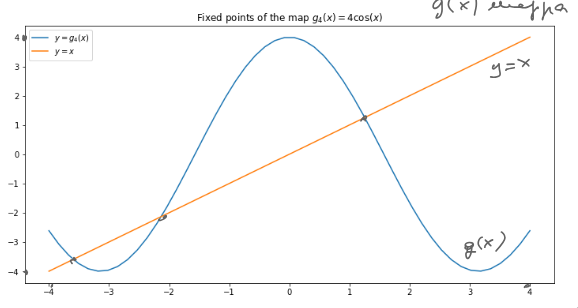
\includegraphics[width=0.5\textwidth]{img/2024-09-28-14-56-48.png}
\end{center}

Come si vede dal grafico della mappa continua $ g(x) $ su $ [-4, 4] $, e' possibile che una mappa abbia piu' di un punto fisso. Per assicurarci l'esistenza di una soluzione unica, dobbiamo aggiugere un'ultima condizione:
\dfn{Mappa contrattiva}{
  Una mappa $ g: D \to D $ si dice \textbf{contrattiva} se esiste $ C < 1 $ tale che:
  \[
    \forall x, y \in D. |g(x)-g(y)| \leq C|x-y|
  \]
  $ C $ e' detta costante contrattiva 
}
Questo significa che per ogni due punti che prendiamo dal dominio, la loro distanza sara' sempre maggiore (o uguale) alla distanza fra i due punti corrispondenti nel codominio. Graficamente (in $ \mathbb{R}^2 $):
\begin{center}
 % 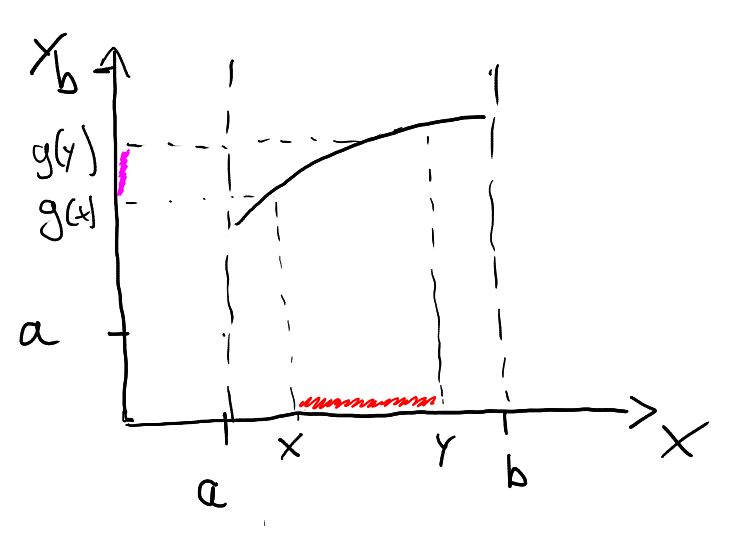
\includegraphics[width=0.5\textwidth]{img/2024-09-28-17-12-32.png}
 no puede soportar este sufrimento
\end{center}
\thm{}{
  Data una mappa contrattiva $ g $ su un intervallo chiuso $ D $, esiste un solo punto fisso $ p $ a cui converge la successione $ x_n $ dove $ x_{k+1} = g(x_k) $, scegliendo $ x_0 $ come qualunque punto in $ D $.
}
\pf{Dimostrazione (singolo punto fisso)}{
Assumiamo che $ g $ abbia piu' di un punto fisso e dimostriamo l'assurdo. Consideriamo il seguente grafico:
\begin{center}
 % 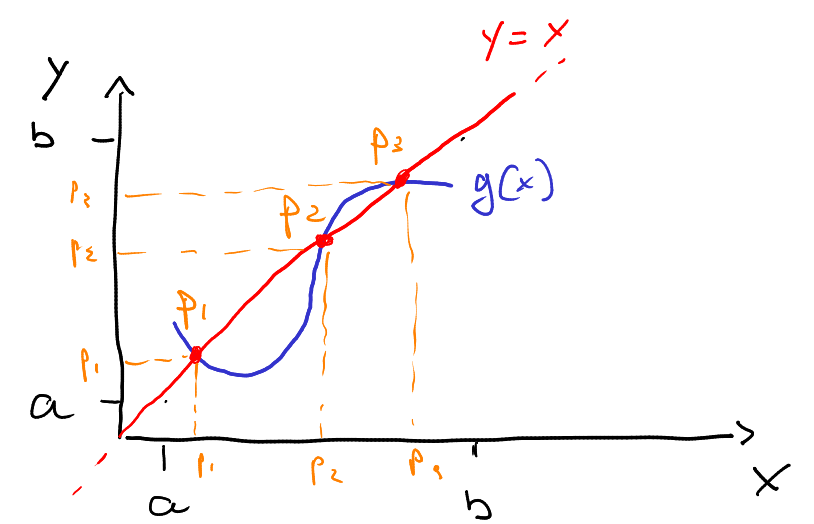
\includegraphics[width=0.5\textwidth]{img/2024-09-28-17-27-59.png}

 no puede soportar este sufrimento
\end{center}
Prendendo due dei punti fissi, $ p_1, p_2 $, notiamo che $ \frac{|g(p_1) - g(p_2)|}{|p_1 - p_2|} = \frac{|p_1 - p_2|}{|p_1 - p_2|} = 1 $, ma dato che la costante $ C $ deve essere minore di $ 1 $, abbiamo dimostrato l'assurdo. 
}
La seconda parte della dimostrazione la vediamo piu' avanti.

\subsubsection{Come controllare se una funzione differenziabile e' una mappa contrattiva}
Nella dimostrazione precedente e' apparsa una forma che somigliava molto a una derivata. Infatti, se la funzione $ g $ e' derivabile possiamo usare il seguente teorema:
\thm{}{
  Se una funzione $ g: [a,b] \to [a,b] $ e' differenziabile e esiste una costante $ C < 1 $ tale che $ \forall x \in [a,b]. |g'(x)|<C $, allora $ g $ e' una \textbf{mappa contrattiva}
}
\pf{Dimostrazione}{
  Per il teorema di Lagrange, $ \forall x < y \in [a,b]. \exists c \in [x,y]. g(y)-g(x) = g'(c)(y-x) $. Quindi, aggiungendo valori assoluti, $|g(y)-g(x)| = |g'(c)|\cdot |y-x| \leq C \cdot |y-x|$ per ipotesi. Quindi, per definizione, $ g $ e' una mappa contrattiva.
}

\subsection{Velocita' del miglioramento dell'approssimazione}
Chiamiamo l'errore assoluto $ |E_k| $ la differenza assoluta fra $ x_k $ e il valore effettivo del punto fisso $ p $.
\mprop{}{
  $ |E_{k+1}| \leq C|E_k| $, quindi 
  \[
  |E_k| = C^k|E_0|
  \]
  Dove $ E_0 = x_0 - p $.
}
Quindi per ogni iterazione, l'errore iniziale diminuisce almeno di un fattore $ C $ (che ricordo e' sempre $ <1 $ quindi e' una cosa buona). Cio' implica che piu' e' piccolo $ C $, piu' ci avviciniamo in fretta a $ p $. 
\pf{Dimostrazione}{
  Per definizione di errore $ E_{k+1} = x_{k+1} - p $, che possiamo riscrivere come $ g(x_k) - g(p) $, quindi per definizione di mappa contrattiva $ |E_{k+1}| = |g(x_k) - g(p)| \leq C|x_k - p| = C|E_k| $. Se sostituiamo $ k = 0 $ abbiamo il caso base:
  \[
  |E_1| = C|x_0 - p|
  \]
  Da cui ricorsivamente: 
  \[
    |E_k| = C\cdot C \cdot ... \cdot C|x_0 - p| = C^k|x_0 - p|
  \]
}

Ora siamo in grado di finire la dimostrazione di prima:
\pf{Diostrazione (convergenza)}{
  Usando la proposizione precedente, $ \lim_{k \to +\infty} |E_k| = \lim_{k \to +\infty} C^k|x_0 - p| = 0 $. Quindi:
  \[
    x_k \xlongrightarrow{k \to +\infty} p
  \]
}

\subsection{Metodo di Newton}
Vediamo ora il metodo di Newton, che rispetto alla bisezione e' generalmente piu' veloce (ma non abbiamo la garanzia). Puo' essere dimostrato come una specifica mappa contrattiva o come approssimazione a linee tangenti, vediamo la prima:\\\\
Prendiamo una funzione differenziabile $ f $ e costruiamole una mappa contrattiva $ g $. Per migliorare l'efficenza, vogliamo fare in modo che la costante $ C $ abbia valore minimo dato un intorno della radice $ r $ di $ f $, come facciamo? Dato che $ C $ assume il valore della derivata massima della mappa, vogliamo fare in modo che la derivata di $ g $ sia minima per quell'intorno. Un modo per fare cio' e' assicurarci che $ g'(r) = 0 $, vediamo come:
\[
  g'(r) = 1 - w'(r)f(r) - w(r)f'(r) = 1 - w(r)f'(r)
\]
dato che $ f(r) = 0 $ per definizione, quindi:
\[
  w(r) = \frac{1}{f'(r)}
\]
Dato che non sappiamo il valore di $ r $, poniamo $ w(x) = \frac{1}{f'(x)} $ per ogni $ x $ nel dominio. Da notare che $ w(x) $ non esiste quando $ f'(x) = 0 $. Facendo cosi', la formula di iterazione diventa:
\[
  x_{k+1} = x_k - \frac{f(x_k)}{f'(x_k)}
\]
che e' la formula per il metodo di Newton.
\section{Risolvere sistemi lineari}
\begin{itemize}
\item Metodi Diretti: +accurati, -efficenti
\item Metodi Iterativi: -accurati, +efficenti
\end{itemize}

\subsection{Fattorizzazione LU}
Per risolvere sistemi lineari, il metodo diretto piu' efficente risulta essere la \textbf{fattorizzazione LU}. Purche' abbia un numero maggiore di operazioni floating-point (flops) rispetto al Gaussian-Jordan, permette di calcolare multiple soluzioni di un sistema $ Ax = b $ decomponendo una sola volta la matrice $ A $. 

\subsubsection{Algoritmo}
Dobbiamo fattorizzare la matrice $ A $ e ottenere due matrici triangolari, una superiore ($ U $) e l'altra inferiore ($ L $). In piu', $ L $ deve avere tutti $ 1 $ sulla diagonale principale. 
\[
A = LU = \begin{pmatrix}
1 & 0 & 0 & 0\\
* & 1 & 0 & 0\\
* & * & 1 & 0\\
* & * & * & 1\\
\end{pmatrix} \cdot \begin{pmatrix}
* & * & * & *\\
0 & * & * & *\\
0 & 0 & * & *\\
0 & 0 & 0 & *\\
\end{pmatrix}
\]

In modo da essere fattorizzabile, $ A $ non deve essere \textit{singolare} ($ detA \neq 0 $) e deve avere i minori principali diversi da 0. Per fare cio', moltiplichiamo la matrice $ A $ per $ n-1 $ matrici $ E_1, E_2, ..., E_{n-1} $ (che per costruzione sono tutte lower) in modo che $ A $ diventi triangolare superiore (sara' il valore di $ U $), mentre $ L $ sara' l'inversa del prodotto $ E_{n-1}\cdot ... \cdot E_2 \cdot E_1 $ (dato che $ L^{-1}A = U $). Quindi per prop dell'inversa $ L = E_1^{-1} \cdot E_2^{-1} \cdot ... \cdot E_{n-1}^{-1} $:
\begin{center}
    no puede soportar este sufrimento
%  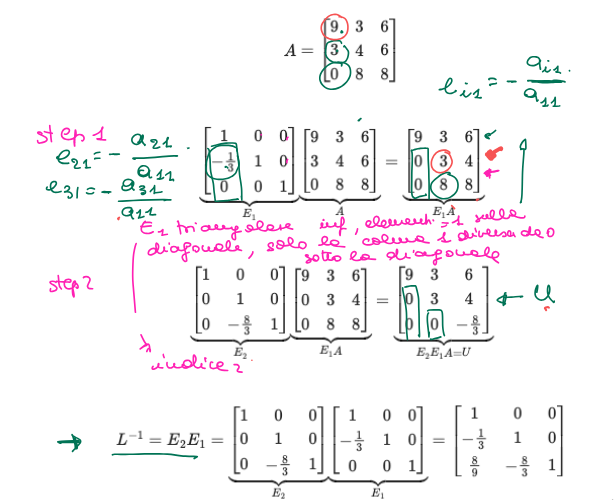
\includegraphics[width=0.5\textwidth]{img/2024-10-04-12-23-45.png}
\end{center}
Dato che $ E_1, E_2, ..., E_{n-1} $ sono triangolari con solo 1 sulla diagonale, per trovare l'inversa basta cambiare di segno i loro valori (tranne gli 1 diagonali). Per evitare di dividere per numeri troppo piccoli durante la costruzione delle matrici lower, e' possibile usare una matrice $ P $ di cambio di righe:
\[
PA = LU \implies A = P^{-1}LU \implies A = PLU
\]

($ P = P^{-1} = P^{T} $). Infine ci resta risolvere il sistema:
\[
Ax = b \implies LUx = b \implies \begin{cases}
Ux = y & \\
Ly = b & 
\end{cases}
\]

Per cui usiamo il metodo di sostituzione avanti, dato che sono sistemi triangolari:
\begin{center}
    no puede soportar este sufrimento
  %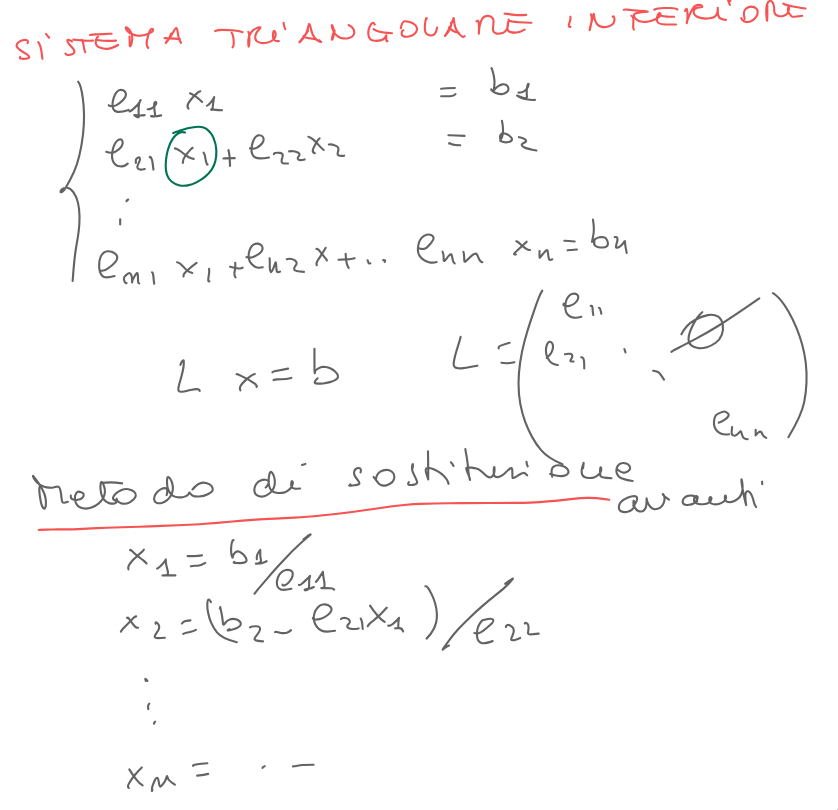
\includegraphics[width=0.5\textwidth]{img/2024-10-14-16-43-56.png}
\end{center}
\subsection{Fattorizzazione di Cholesky}
Si puo' usare solo nel caso speciale in cui $ A $ sia \textbf{definita semi-positiva}:
\dfn{Matrice semi-definita positiva}{
  $ A $ $ n \times n $ simmetrica e' \textbf{semi-definita positiva} se $ \forall x \in \mathbb{R}^n: $
  \[
  x^T A x \geq 0
  \]
}

Per cui vale:
\mprop{Autovalori di matrici semi-definite positive}{
 Data una matrice $ A $ semi-definita positiva, ogni autovalore di $ A $ e' positivo o nullo
}

Grazie a queste proprieta', possiamo dire che $ \exists L: $
\[
A = L \cdot L^T
\]
e trovarlo e' circa due volte piu' efficente rispetto a LU.

\section{Approssimazione}
\subsection{SVD}
\nt{
  Fonti: 
  \begin{itemize}
      \item \href{https://www.youtube.com/watch?v=vSczTbgc8Rc}{Visualizzazione geometrica}
      \item \href{https://www.youtube.com/watch?v=vSczTbgc8Rc}{Visualizzazione vettori ortogonali e dimostrazione minimo quadrato}
      \item \href{https://gregorygundersen.com/blog/2018/12/20/svd-proof}{Dimostrazione SVD}
  \end{itemize}
}
Prima di iniziare ad introdurre metodi di approssimazione, e' necessario esplorare uno dei teoremi finali dell'algebra lineare: la \textbf{SVD} (Singular Value Decomposition). Questo teorema sara' fondamentale per descrivere vari modelli di ottimizzazione e approssimazione per motivi che vedremo dopo.\\
\\
\subsubsection{Introduzione}
Un modo per arrivare alla SVD e' porci la seguente domanda: data una matrice $ A \in M(\mathbb{R})_{n \times m} $, esistono $ m $ vettori ortonormali in $ \mathbb{R}^m $ la cui immagine e' sempre un insieme di $ m $ vettori ortogonali (se $ m > n $ allora $ m -n $ vettori dell'immagine saranno nulli) in $ \mathbb{R}^n $? Proviamo a scrivere la domanda in modo piu' matematico:
\[
  \exists V \in M(\mathbb{R})_{m}, U \in M(\mathbb{R})_n, \Sigma \in M(\mathbb{R})_{n \times m}. V, U \text{ ortonormali, } \Sigma \text{ diagonale (rettangolare)}. \forall A \in M(\mathbb{R})_{n \times m}:
\]
\[
 AV = U\Sigma
\]
dove $ V $ ha come colonne i vettori ortonormali del dominio, $ U $ ha come colonne vettori ortonormali (se $ n > m $ le ultime $ n-m $ colonne non importano e possono essere nulle) che moltiplicate per i corrispondenti scalari sulla diagonale della matrice $ \Sigma $ formano l'immagine ortogonale di $ V $. Dato che $ V $ e' ortonormale, posso riscrivere l'equazione come scomposizione di $ A $:
\[
A = U\Sigma V^T
\]
Questa e' la scomposizione di cui la SVD ci assicura l'esistenza per qualsiasi matrice $ A $, formalmente:
\thm{Singular Value Decomposition}{
  Per qualsiasi $ A \in M(\mathbb{R})_{n \times m} $, esistono:
  \begin{itemize}
    \item $ U $ ortonormale $ n \times n $
    \item $ V $ ortonormale $ m \times m $
    \item $ \Sigma $ rettangolare diagonale $ n \times m $
  \end{itemize}
  Tali che:
  \[
    A = U\Sigma V^T
  \]
}
\mlenma{Lemma 1}{
  Per una qualsiasi matrice $ A \in M(\mathbb{R})_{n \times m} $, si ha che:
  \begin{itemize}
    \item $ A^T A \in M(\mathbb{R})_n $ semidefinita positiva
    \item $ A A^T \in (\mathbb{R})_m $ semidefinita positiva
  \end{itemize}
}
\pf{}{
  Dimostra (forse)
}

\pf{Dimostrazione SVD}{
  Sia $ A \in M(\mathbb{R})_{n \times m} $. Per Lemma 1, sappiamo che $ A^T A $ e' una matrice semidefinita positiva, quindi, per il teorema spettrale, puo' essere scomposta come:
  \[
  A^T A = V \Lambda V^T
  \]
  dove $ V \in M(\mathbb{R})_m $ e' una matrice ortonormale e $ \Lambda \in M(\mathbb{R})_m $ e' la matrice diagonale di autovettori ordinati $ \lambda_1 \geq ... \geq \lambda_m $ tali che $ Av_1 = \lambda_1 v_1 $. Definiamo ora $ n $ vettori $ u_i $ nel seguente modo, dove $ \sigma_i = \sqrt{\lambda_i} $:
  \[
  u_i = \begin{cases}
  \frac{Av_i}{\sigma_i} & \lambda_i \neq 0 \\
  \underline{0} & \lambda_i = 0
  \end{cases} 
  \]
  Dato che $ A^T A $ ha lo stesso rango di $ A $ (dim. nella fonte), se $ A $ ha rango massimo allora $ \forall i. \sigma_i > 0 $ (perche' si puo' dimostrare che $ A^T A $ diventa \textbf{definita} positiva); se $ r = rank(A) < min(n, m) $, allora gli ultimi $ min(n, m) - r $ valori singolari saranno nulli. (Da riguardare perche non sono sicurissimo)
  Si puo' dimostrare che $ u_i $ sono autovettori di $ A A^T $:
  \begin{align*}
    A A^T u_i &= A A^T \frac{Av_i}{\sigma_i} \\
    &= A \frac{\sigma_i^2 v_i}{\sigma_i} \\
    &= \sigma^2\frac{A v_i}{\sigma_i} \\
    &= \sigma^2 u_i
  \end{align*}
  E che sono unitari:
  \begin{align*}
    u_i^T u_i &= \frac{v_i^T A^T}{\sigma_i} \frac{Av_i}{\sigma_i} \\
    &= \frac{v_i^T \sigma^2 v_i}{\sigma^2} \\
    &= v_i^T v_i = 1
  \end{align*}

  Essendo autovettori unitari di una matrice semidefinita positiva ($ A A^T $), la matrice $ U \in M(\mathbb{R})_n $ che ha come colonne $ u_i $ e' ortonormale. Usando le matrici possiamo scrivere:
  \[
   Av_i = \sigma_i u_i \implies AV = U \Sigma 
  \]
  dove $ \Sigma \in M(\mathbb{R})_{n \times m} $ ha sulla diagonale $ min(n, m) $ valori singolari ($ \sigma_1,...,\sigma_{min(n, m)} $) e il resto e' 0.
  \[
  A = U \Sigma V^T
  \]
}

\subsubsection{Interpretazione geometrica}
Questa scomposizione puo' essere interpretata in modo geometrico. Immaginiamo di moltiplicare un vettore $ x $ per la scomposizione di $ A $:
\begin{itemize}
  \item La matrice $ V^T $, essendo ortonormale, applica una rotazione a $ x $ senza variarne il modulo. Essendo trasposta, che per le matrici ortonormali corrisponde con l'inversa, al posto di spostare i vettori base ai vettori di $ V $ fa il contrario.
  \item La matrice $ \Sigma $ puo' essere scomposta in due parti:
    \begin{itemize}
      \item La matrice $ m \times m $ diagonale, che ha come valori diagonali gli $ m $ valori singolari. Dato che e' diagonale, applica solo un'allungamento/restrizione di x ruotato.
      \item Una matrice $ n \times m $ rettangolare diagonale con solo valore $ 1 $. Serve per portare il vettore nel nuovo spazio vettoriale. 
      \begin{center}
        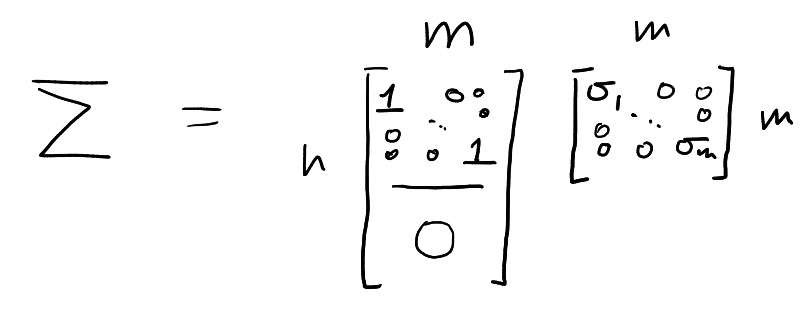
\includegraphics[width=0.5\textwidth]{img/2024-11-20-17-27-02.png}
      \end{center}
    \end{itemize}
  \item Infine la matrice $ U $ ortonormale ruota il vettore nello spazio del codominio $ \mathbb{R}^n $, spostando la base sui vettori di $ U $.
\end{itemize}

\ex{Mappa da sfere a elissoidi}{
  Consideriamo una cironferenza unitaria in $ \mathbb{R}^2 $:
\begin{center}
  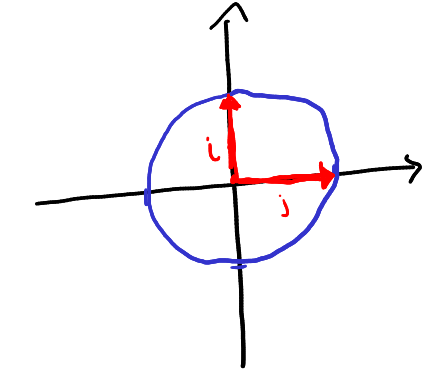
\includegraphics[width=0.3\textwidth]{img/2024-11-21-09-53-22.png}
\end{center}
Applichiamo la trasformazione lineare definita dalla matrice $ A \in M(\mathbb{R})_{3 \times 2} $. Come abbiamo visto, qualunque matrice puo' essere scomposta come due matrici di rotazione e una di "allungamento". Vediamo i vari passaggi:
\begin{itemize}
  \item Applicando la prima rotazione, la nostra figura non cambia dato che e' una circonferenza:

\begin{center}
  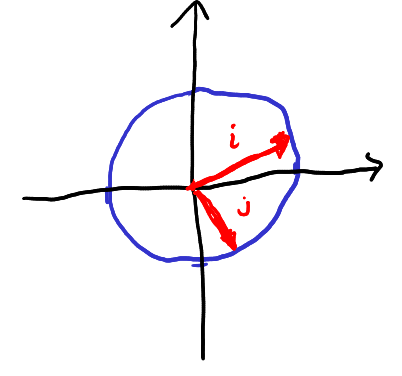
\includegraphics[width=0.3\textwidth]{img/2024-11-21-10-02-10.png}
\end{center}
  \item Moltiplicando per la matrice diagonale, la circonferenza viene allungata lungo due assi principali (i vettori della base canonica che sono stati roteati da $ V^T $). Abbiamo quindi un'ellisse:

\begin{center}
  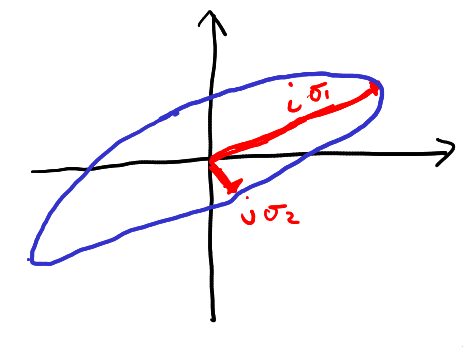
\includegraphics[width=0.3\textwidth]{img/2024-11-21-10-02-40.png}
\end{center}
  \item Spostiamo l'ellisse in $ \mathbb{R}^3 $:

\begin{center}
  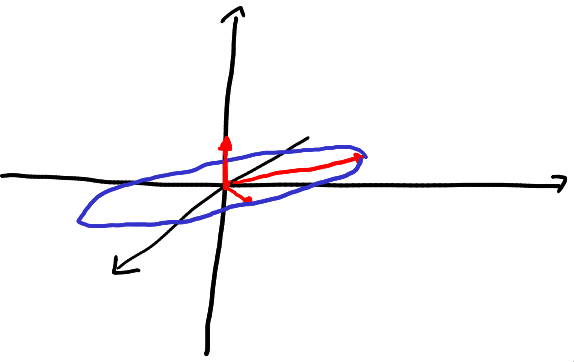
\includegraphics[width=0.3\textwidth]{img/2024-11-21-10-03-11.png}
\end{center}
  \item Manca solo l'ultima rotazione applicata da $ U $, questa volta in $ 3 $ dimensioni:

\begin{center}
  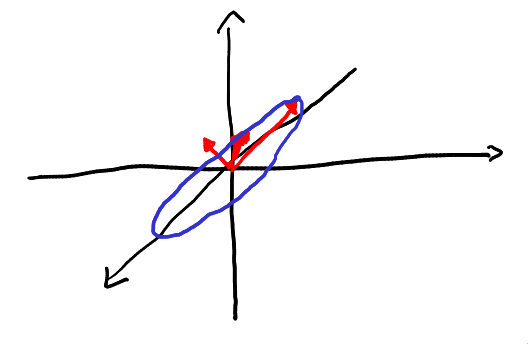
\includegraphics[width=0.3\textwidth]{img/2024-11-21-10-03-38.png}
\end{center}
  
\end{itemize}
  Per questo motivo, possiamo dire che le matrici $ n \times m $ trasformano sfere in $ \mathbb{R}^m $ in elissoidi a $ n $ dimensioni.
}

Quindi i \textbf{valori singolari} $ \sigma_1,...,\sigma_{min(n, m)} $ sono i coefficenti scalari che moltiplicano i vettori lungo $ min(n, m) $ assi ortogonali. 

\subsubsection{Applicazioni}
La SVD e' uno strumento utilizzato moltissimo per problemi di ottimizzazione e di aprossimazione, in quanto e' applicabile universalmente e fornisce informazioni molto importanti per l'analisi dei dati. La lista ordinata in modo discendente rispetto a quanto la matrice "allunga" i vettori lungo una certa direzione (vettori singolari destri e sinistri ???) e' utilizzata per la PCA (Principal Component Analisis ???) e per l'aprossimazione di matrici. Inoltre, la SVD e' utilizzata per risolvere il problema dei minimi (o massimi) quadrati, come vedremo prossimamente.
